\chapter{Zorro Implementation}
\label{ch:Zorro}

With the capabilities provided by Hackystat and SDSA, as part of 
my dissertation research, I implemented the Zorro software system 
for the automation of Test-Driven Development (TDD) behavior 
inference. As illustrated in Figure \ref{fig:ZorroInfrastructure}, 
Zorro is a specialization of the SDSA framework for TDD, supported 
by Hackystat. Zorro not only uses Hackystat's generic services such 
as sensor data collection and persistence, but also contributes 
new functionalities to Hackystat. Zorro defines
several analyses and telemetry streams to study TDD using activities 
collected in development environment tools. This chapter starts with 
Zorro's extensions to the Hackystat and SDSA frameworks, followed 
by a collection of Zorro's TDD analyses.

\section{Extensions to Hackystat's Data Collection}
\label{sec:Zorro-Hackystat}

\begin{comment}
A nice thing about Hackystat is that numerous sensors have already 
been developed. Over two dozen sensors are currently available, including 
sensors for IDEs (Emacs, JBuilder, Eclipse, Vim, VisualStudio, Idea), 
configuration management (CVS, Subversion), testing and coverage (JUnit, 
CppUnit, Emma, JBlanket), and so forth. Though availability of tool 
supports gives developers the freedom to choose the right tool for 
a given task without losing process metric data, it is also difficult 
to automate the recognition. Thus, to begin with, Zorro requires that the TDD development 
must be done in a supported IDE. Under this premise, Zorro uses the 
sensor data collected in the IDE, and ignores other development activities
that are probably irrelevant to TDD. 
\end{comment}

Zorro has special requirements for Hackystat sensors that are 
responsible for collecting software metrics. In order to 
partition development streams and recognize TDD development 
behaviors, certain software development activities must be 
collected. Table \ref{tab:Zorro.Sensors} contains a list of the 
required development activities including edit, compile, test, 
switch file, and refactor. The ``DevEvent'' is 
a sensor data type defined in Hackystat to represent these 
kinds of development activities using the combination of ``Type'' 
and ``Subtype'' attributes. In addition, DevEvent defines a special 
attribute named ``PropertyMap'' to hold the required metrics, which 
are listed in the ``Product or Process Metrics'' column of 
Table \ref{tab:Zorro.Sensors}. Note that DevEvent does
not have the ``Kind'' attribute as you can see in 
Table \ref{tab:Zorro.Sensors}. It is for the sake of 
clarification for sensor developers to determine
what metrics are mandatory. For instance, if a test is
edited, the ``current-test-method'' and ``current-test-assertion'' 
metrics must be collected in addition to other metrics 
required for editing activities on production code. 

\begin{table}[htbp]
\centering
  \caption{Sensor Data Types Required by Zorro}
  \begin{tabular}{|p{2cm}|l|p{2.5cm}|l|p{6cm}|} \hline 
   Development & \multicolumn{2}{c|}{DevEvent} & \multicolumn{2}{c|}{Product or Process Metrics} \\ \cline{2-5}
   Activity & Type & Subtype & Kind & Names \\ \hline
   Edit &  Edit & StateChange and Save   & Document   & current-size \\ \cline{4-5}
        &       &                        & Production & current-size, class-name, 
                                                       current-methods, current-statements \\
                                                  \cline{4-5}
        &       &                        &  Test      & current-size, class-name, current-methods, 
                                                        current-statements, current-test-methods, 
                                                        current-test-assertions \\ \hline
   Compile     & Build    & Compile     &          &  success, error   \\ \hline   
   Test        & Test     & UnitTest    &          &  test-name, success, test-count, test-indice, 
                                                     elapsed-time, run-time \\ \hline 
   Switch File  & Edit   & BufferTransition &     & from-buff-name, to-buff-name \\ \hline                                                     
   Refactor    & Edit     & ProgramUnit & Unary    &  op (add or remove), unit-name, unit-type, 
                                                      language\\ \cline{4-5}
               &          &             & Binary   &  op (rename or move), unit-type, from-unit-name,
                                                      to-unit-name, language\\ \hline              
  \end{tabular}
  \label{tab:Zorro.Sensors}
\end{table}

These development activities are language and IDE independent. 
I wrote a sensor for Eclipse to gather these activities and more 
recently wrote a similar sensor for Visual Studio .NET. It 
should be possible to enhance a wide range of IDEs to collect 
necessary development activities for Zorro's automated TDD 
behavior inference.  

\section{Extensions to SDSA}
Zorro is a specialization of SDSA for automated inference of 
development behaviors of TDD. Figure \ref{fig:Zorro-SDSA-Workflow} 
illustrates how Zorro specializes SDSA. First, Zorro requires 
certain types of development activities, as described in 
Section \ref{sec:Zorro-Hackystat}. Thus, the development 
stream in Zorro is a special type of software development stream, which 
collects specific development activities useful for TDD recognition.
Second, Zorro uses the ``test pass'' tokenizer defined in the SDSA 
framework to partition the development stream. Last, a special set 
of rules are defined in Zorro to infer TDD development behaviors. In 
this section, I will describe Zorro's specialization of SDSA in detail.
\begin{figure}[htbp]
  \centering
  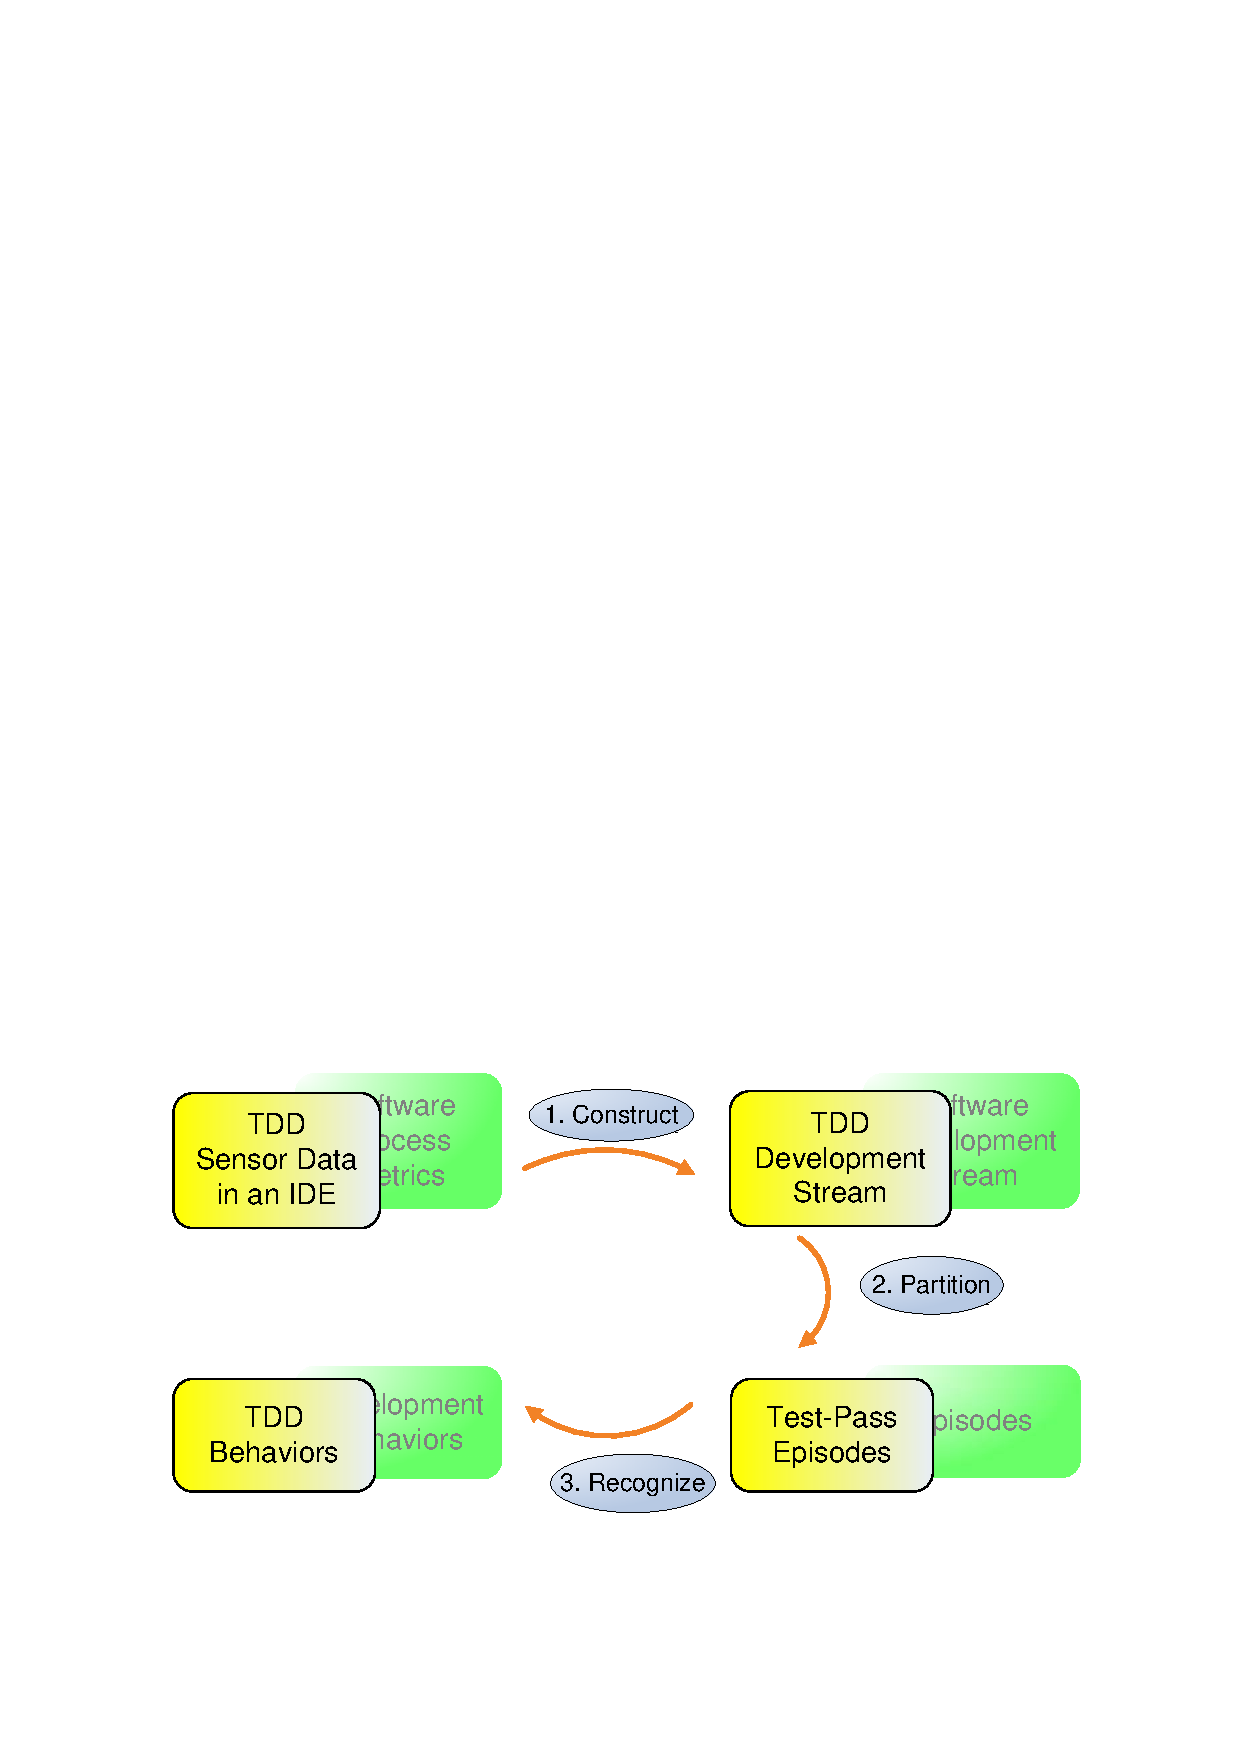
\includegraphics[width=0.8\textwidth]{figs/Visio-Zorro-SDSA-FlowChart}
  \caption{Zorro's Extensions to the SDSA Framework}
  \label{fig:Zorro-SDSA-Workflow}
\end{figure}

\subsection{Zorro Development Stream}
Edit, compile, test, switch file, and refactor are five types
of development activities required by Zorro. Though other 
development activities such as command line invocations can be 
conducted by developers, Zorro does not include them in
the development stream because they are not useful for 
recognition of TDD. The following code shows how Zorro 
constructs a development stream using SDSA. 
\begin{verbatim}
   DevelopmentStream stream = 
       new DevelopmentStream(project, user, startDay, endDay);
   stream.addSubstream(new EditStream(user));
   stream.addSubstream(new BuffTransStream(user));
   stream.addSubstream(new RefactoringStream(user));
   stream.addSubstream(new UnitTestStream(user));
   stream.addSubstream(new CompilationStream(user));
   stream.assemble(); 
\end{verbatim}
This piece of code instantiates a ``DevelopmentStream'' 
for a given project, a project member, and a specified time 
period indicated by the start day and the end day. It assembles
five action streams together to create the TDD development 
stream. 

\subsection{TDD Development Stream Partition}
Zorro uses the ``test pass'' tokenizer defined in the SDSA 
framework (see Section \ref{sec:SDSA-Construction}). As a 
result, a development stream is partitioned into a sequence 
of ``test pass'' episodes all of which end with successful 
unit test invocations. Figure \ref{fig:SDSA-Example} 
illustrates this process.

Before we move on, let's pause a while and think about the 
methods we are using. The development stream in Zorro 
contains five types of development activities that occur 
in an IDE when a developer is programming. These 
activities are not TDD specific. Moreover, the ``test
pass'' tokenizer is used to divide the TDD development stream
into ``test pass'' episodes. Again, the ``test pass'' tokenizer 
is not TDD specific and a developer might invoke tests no matter what
development methods he/she is using. Given this, how can we 
recognize development behaviors in TDD?  Can we use a dedicated 
tokenizer for TDD such as a ``TDD Iteration'' tokenizer? 

Recall that the order of programming in TDD is 
``Red/Green/Refactor''. If a developer programs in TDD, tests 
should be invoked one or more times. Given a task from the To-Do 
list (see Section \ref{sec:related-tdd}), a developer quickly 
writes a test and then invokes it. He or she will get a red
bar if the test fails. After implementing functional code 
for the task, he or she will invoke the test again to see it 
pass. Therefore, when the ``test pass'' tokenizer 
is used, we will get an episode containing the ``Red/Green'' 
development portion of a TDD cycle. If there is any redundancy
in the code, the developer will refactor it and then invoke
the test again. As a result, we will get another episode 
containing the ``Refactoring'' portion of a TDD cycle. If we 
can successfully recognize the ``test first'' behavior in the 
first episode and the ``refactoring'' behavior in the second 
episode, then we will be able to recognize TDD development 
behavior using the divide-conquer method. This shows that 
the ``test pass'' tokenizer is sufficient for recognition of 
development behaviors in TDD. The first question is answered. 

Can we have a ``TDD Iteration'' tokenizer? The answer is 
probably no. First, detecting refactoring development 
behaviors is hard. It is hard to tell whether a developer
is adding new code or refactoring for simpleness and clarification.
Second, as we have discussed in Chapter \ref{ch:Introduction}, 
developers may or may not conform to TDD, the Red/Green/Refactor 
cycle may not exist sometimes. Fortunately, the test pass tokenizer 
is sufficient for us to find the boundary of TDD's 
Red/Green/Refactor cycles as we just showed in last 
paragraph. 

\subsection{Inference of TDD Development Behavior}
\label{sec:ZorroBehaviorCategory}

%% Zorro use successful test invocations as the token to 
Zorro also extends SDSA with a set of rules that enable instances 
of test pass episodes to be classified as one of 22 episode types.  
Table \ref{tab:Zorro.Categories} lists these episode types,
their definition in terms of their internal patterns of
development activities, and an indication of their TDD 
conformance. 
\begin{sidewaystable}[htbp]
\centering
  \caption{Zorro episode types, definitions, and TDD conformance}
  \begin{tabular}{|l|p{18.5cm}|l|}
  \hline
   \textbf{ID}  & \textbf{Definition}   & \textbf{TDD Conformant} \\ \hline
   \multicolumn{3}{|l|}{\textbf{Test First}} \\ \hline
   TF-1 & Test creation $\rightarrow$ Test compilation error $\rightarrow$ 
          Code editing $\rightarrow$ Test failure $\rightarrow$ Code editing 
          $\rightarrow$ Test pass & Yes \\ \hline
   TF-2 & Test creation $\rightarrow$ Test compilation error $\rightarrow$ 
          Code editing $\rightarrow$ Test pass & Yes \\ \hline
   TF-3 & Test creation $\rightarrow$ Code editing $\rightarrow$ Test failure 
          $\rightarrow$ Code editing $\rightarrow$ Test pass    & Yes \\ \hline
   TF-4 & Test creation $\rightarrow$ Code editing $\rightarrow$ Test pass      
        & Yes \\ \hline

   \multicolumn{3}{|l|}{\textbf{Refactoring}} \\ \hline
   RF-1 & Test editing $\rightarrow$ Test pass  & Context sensitive \\ \hline
   RF-2 & Test refactoring operation $\rightarrow$ Test pass    & Context sensitive \\ \hline
   RF-3 & Code editing (number of methods or statements decrease) $\rightarrow$ Test pass       
        & Context sensitive \\ \hline
   RF-4 & Code refactoring operation $\rightarrow$ Test pass    & Context sensitive \\ \hline
   RF-5 & [Test Editing \&\& Code editing (number of methods or 
          statements decrease)]+ $\rightarrow$ Test pass        
        & Context sensitive \\ \hline
   
   \multicolumn{3}{|l|}{\textbf{Test Addition}} \\ \hline
    TA-1        & Test creation $\rightarrow$ Test pass & Context sensitive \\ \hline
    TA-2        & Test creation $\rightarrow$ Test failure $\rightarrow$ Test editing 
            $\rightarrow$ Test pass     
          & Context sensitive \\ \hline

   \multicolumn{3}{|l|}{\textbf{Regression}} \\ \hline
   RG-1 & Non-editing activities $\rightarrow$ Test pass        & Context sensitive \\ \hline
   RG-2 & Test failure $\rightarrow$ Non-editing activities $\rightarrow$ Test pass     
        & Context sensitive \\ \hline

   \multicolumn{3}{|l|}{\textbf{Code Production}} \\ \hline
    CP-1        & Code editing (number methods unchanged, statements increase) 
            $\rightarrow$ Test pass     
          & Context sensitive \\ \hline
    CP-2        & Code editing (number methods /statements increase slightly 
            (source code size increase $\leq$ 100 bytes) $\rightarrow$ Test pass        
          & Context sensitive \\ \hline
    CP-3        & Code editing (number methods /statements increase significantly 
            (source code size increase $>$ 100 bytes) $\rightarrow$ Test pass   
          & No \\ \hline

    \multicolumn{3}{|l|}{\textbf{Test Last}} \\ \hline
    TL-1        & Code editing $\rightarrow$ Test editing $\rightarrow$ Test pass       & No \\ \hline
    TL-2        & Code editing $\rightarrow$ Test editing $\rightarrow$ Test failure 
            $\rightarrow$ Test editing $\rightarrow$Test pass   
          & No \\ \hline

    \multicolumn{3}{|l|}{\textbf{Long}} \\ \hline
    LN-1        & Episode with many activities ($>$ 200) $\rightarrow$ Test pass        & No \\ \hline
    LN-2        & Episode with a long duration ($>$ 30 minutes) $\rightarrow$ Test pass & No \\ \hline

    \multicolumn{3}{|l|}{\textbf{Unknown}} \\ \hline
    UN-1        & None of the above $\rightarrow$ Test pass     & No \\ \hline
    UN-2        & None of the above     & No \\ \hline
  \end{tabular}
  \label{tab:Zorro.Categories}
\end{sidewaystable}

Zorro organizes the 22 episode types into eight categories: Test First
(TF), Refactoring (RF), Test Last (TL), Test Addition (TA), Regression
(RG), Code Production (CP), Long (LN), and Unknown (UN). All of these
episode types (except UN-2) always end with a ``Test Pass'' event, since 
that is the episode boundary condition.  UN-2 is provided as a way to 
classify a development stream where there is no unit testing at all.

\subsubsection{Test First}
``Test First'' can be seen as the Red/Green portion of a TDD cycle.
In a ``Test First'' episode, a test method or assertion statement is 
created first, followed by production code editing. Depending on 
compilation and test invocation results, an episode can be one of the
four types: TF-1, TF-2, TF-3, or TF-4, as illustrated in 
Table \ref{tab:Zorro.Categories}. 

\subsubsection{Refactoring}
Refactoring behaviors in reality are a bit complicated to recognize 
automatically because developers can refactor code in many different 
ways. A simple scenario of refactoring is to change a method implementation 
without changing its input and output. To accomplish this, the developer 
can edit code directly or abstract a new method from it for reuse. 
Directly matching the patterns of refactoring behaviors is hard, but 
we can observe them indirectly. 
First of all, there should be no test created. Second, code being 
refactored should not increase in size. If it does, the increase 
should be relatively small. With these two principles in mind, we can define
rules to infer refactoring behaviors. Table \ref{tab:Zorro.Categories}
lists five kinds of refactoring episodes: RF-1, RF-2, RF-3, RF-4, and 
RF-5. Among them, RF-1 and RF-2 are refactoring on test, RF-3 and RF-4 
are refactoring on production code, and RF-5 defines mixed refactoring 
on both test and production code. 

\subsubsection{Test Addition}
If you are a TDD developer, you probably have never heard of ``Test Addition''
since Beck did not explicitly define it in \cite{Beck:03}. However,
you may occasionally add a test that does not drive implementation of
new production code, thus ``Test Addition'' exists even if you do not
realize it. It is fundamentally different from the refactoring behavior 
on test code because test methods and assertion statements are added. 
Zorro defines two types of ``Test Addition'' behaviors: TA-1 and TA-2.

\subsubsection{Regression}
It is always a good habit to run existing tests before adding any new 
code into the system, especially at the beginning. This development behavior
is called the regression test. The tests may fail due to problems such 
as incorrect environment settings, so the regression behavior has two 
categories: RG-1 and RG-2. 

\subsubsection{Code Production}
Recall that developers might not develop software 
following the pattern of Red/Green/Refactor all the time, as we discussed
in Chapter \ref{ch:Introduction}. Also, some developers may use 
other software development methods, such as Test Last Programming. 
For example, it is possible that a big chunk of production code can be inserted 
into the system without corresponding tests. Although tests
are invoked in the end, the development behavior is actually about 
writing production code. Zorro therefore defines ``Code Production'' to 
classify this variety of development behaviors. Depending on the size increase 
of production code, ``Code Production'' has three types: CP-1 (statement 
increase only), CP-2 (small code increase), and CP-3 (big production code 
increase).

\subsubsection{Test Last}
``Test Last'' is not a development behavior of TDD, but it is useful
to define it. Researchers have compared TDD to Test Last Programming or
Iterative Test Last \cite{Erdogmus:05,Matjaz:03}. If Zorro differentiates 
TDD from ``Test Last'', it can greatly help empirical researchers to study
TDD in practice.  ``Test First''  is opposed to ``Test Last'' where a test 
is created after production code implementation. ``Test Last'' has two
types: TL-1 and TL-2, however, the difference between the two types is 
very small. 

\subsubsection{Long}
Development behaviors in long episodes such as ones with too many 
development activities or ones that last a very long time (over 30 minutes)
are very hard to recognize. Therefore, Zorro does not infer development 
behaviors of long episodes. This is acceptable because iterations of TDD 
should be just seconds or minutes in duration\cite{Beck:01}. If an episode 
is very long, it is very likely not to be TDD conformant. 

\subsubsection{Unknown}
The last type of development behavior is ``Unknown''.
UN-2 is defined to classify development streams that do not have
any successful unit test invocation. UN-1 is defined to incorporate 
the situation that the rule set is insufficient, which is very rare but 
we can not exclude it. 

\subsection{TDD Conformance}
\label{sec:Zorro-TDDConformance}
% Two-way heuristic  
Once each episode instance has been assigned an episode type, the final 
step in the Zorro classification process is to determine the TDD 
conformance of that instance. Table \ref{tab:Zorro.Categories} shows 
that instances of some of the episode types are easy to characterize. 
For example, every instance of a ``Test First'' episode type is automatically 
TDD conformant, and every instance of a ``Test Last'', ``Long'' and 
``Unknown'' episode type is automatically not TDD conformant.

Interestingly, several of the episode types, such as ``Refactoring'', ``Test
Addition'', ``Regression'', and certain ``Code Production'' are ambiguous: in
certain contexts, they could be TDD conformant, while in others they could
be TDD non-conformant. This is because, for example, ``Refactoring'' can
legitimately occur while a developer is either doing TDD or some different 
development approach, such as Test Last Programming.  In
order to classify instances of these episode types, Zorro applies the
following heuristic: if a sequence of one or more ambiguous episodes are
bounded on both sides by TDD non-conformant episodes, then these ambiguous
episodes types are classified as TDD non-conformant.

To make this clear, let's consider some examples, such as the episode
sequence [TF-1, RF-1, CP-1, TF-2]. In this sequence, Zorro 
classifies the ambiguous episodes (RF-1 and CP-1) as TDD conformant, 
since they are surrounded by TDD conformant episode types (TF-1 and TF-2). 
Figure \ref{fig:Zorro-EpisodeSequence-ExampleA} illustrates this scenario.  
In Figure \ref{fig:Zorro-EpisodeSequence-ExampleA}, a rectangle with 
letters represents an episode, and it is painted with green background 
if it is TDD conformant according to the heuristic. 
\begin{figure}[htbp]
  \centering
  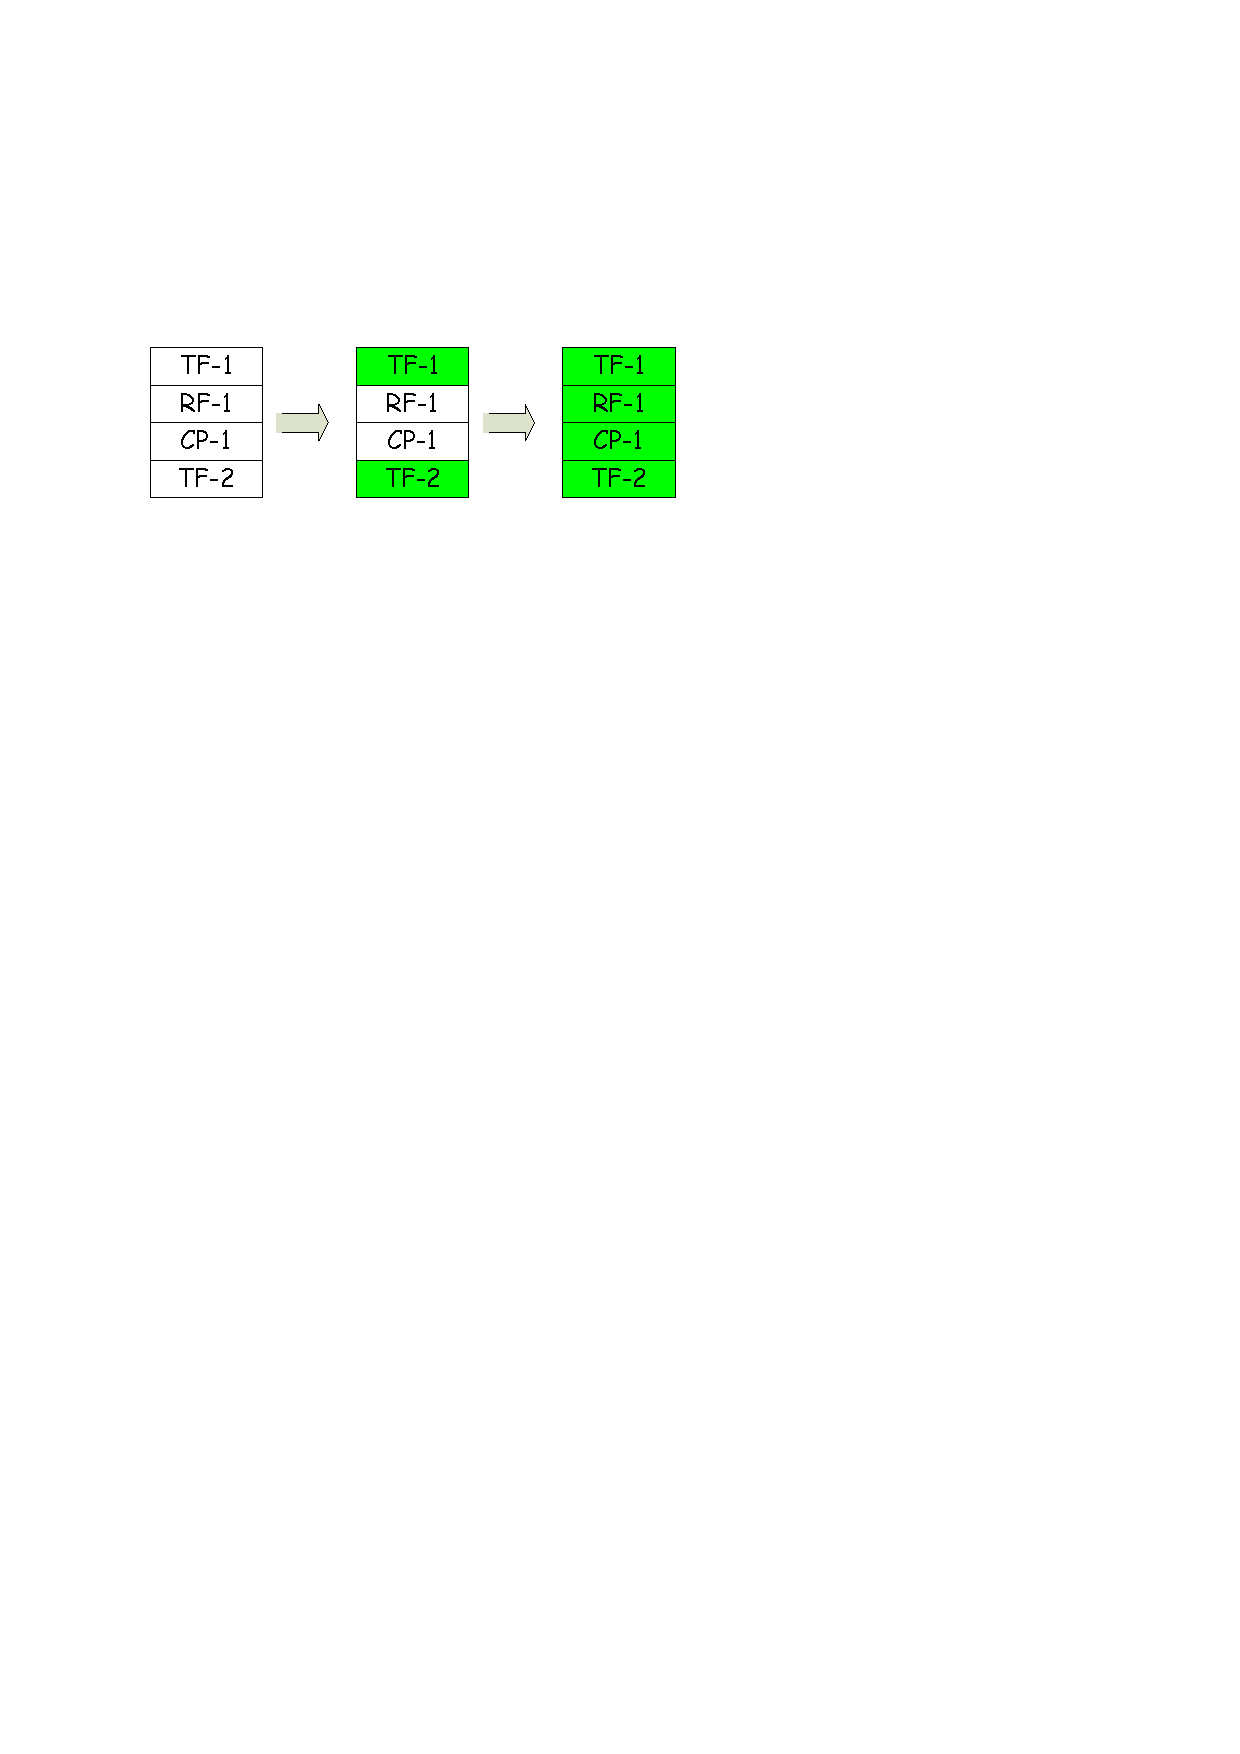
\includegraphics[width=0.4\textwidth]{figs/Visio-Zorro-Heuristic-Example1}
  \caption{Episode Sequence Example A}
  \label{fig:Zorro-EpisodeSequence-ExampleA}
\end{figure}

Now consider the sequence: [TL-1, RF-1, CP-1, TL-2].  In this sequence, 
Zorro classifies the same two ambiguous episodes (RF-1 and CP-1) as TDD 
non-conformant, since they are surrounded by TDD non-conformant episode types 
(TL-1 and TL-2). This scenario is illustrated in Figure 
\ref{fig:Zorro-EpisodeSequence-ExampleB} where an episode is painted
with red background if it is TDD non-conformant. 
\begin{figure}[htbp]
  \centering
  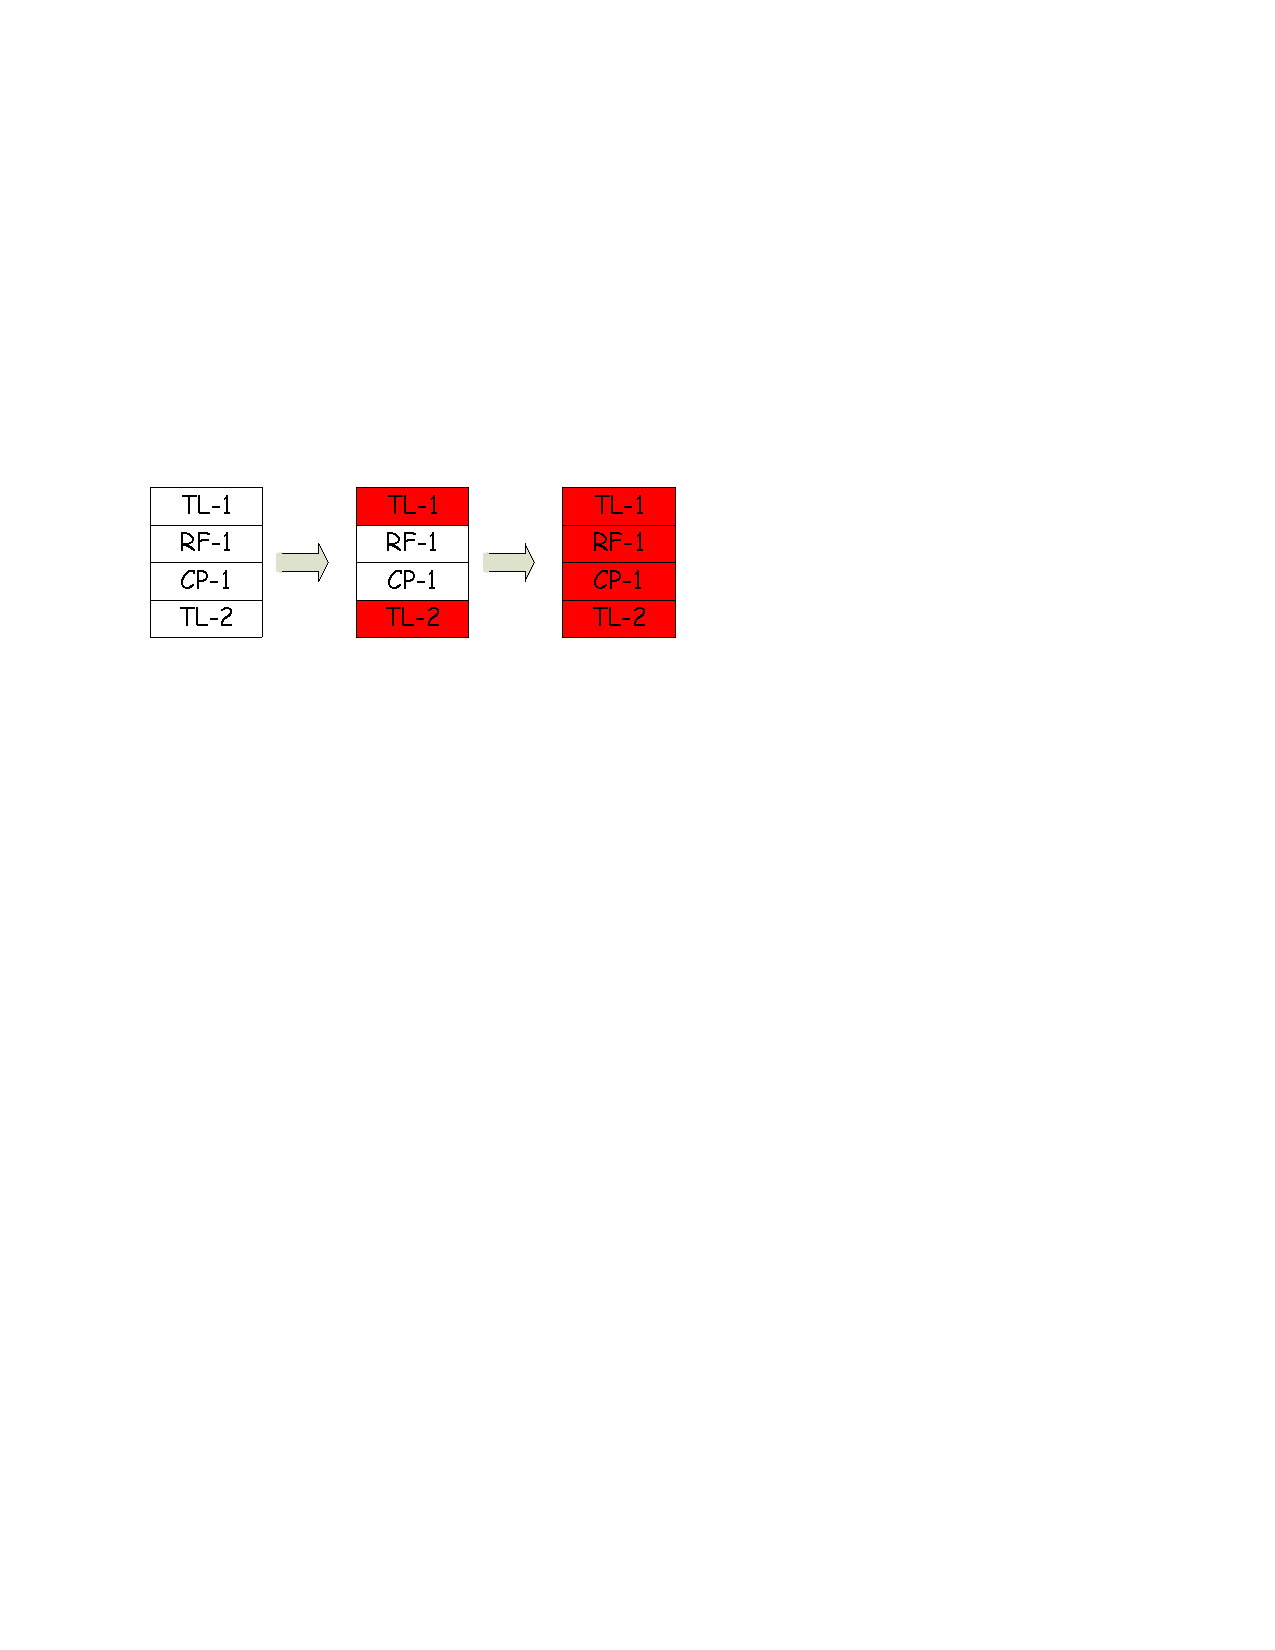
\includegraphics[width=0.4\textwidth]{figs/Visio-Zorro-Heuristic-Example2}
  \caption{Episode Sequence Example B}
  \label{fig:Zorro-EpisodeSequence-ExampleB}
\end{figure}

Now consider a sequence like: [TL-1, RF-1, CP-1, TF-1] illustrated 
in Figure \ref{fig:Zorro-HeuristicAlgorithm}. Here, the two ambiguous 
episodes (RF-1 and CP-1) are surrounded on one side by an unambiguously 
TDD conformant episode (TL-1) and on the other side by an unambiguously 
TDD non-conformant episode (TF-1).  In this case, Zorro's rules 
could implement an ``optimistic'' classification, and assign the
ambiguous episodes as TDD, or a ``pessimistic'' classification, and 
assign the ambiguous episodes as TDD non-conformant. 
Figure \ref{fig:Zorro-HeuristicAlgorithm} illustrates both of heuristics. 
\begin{figure}[htbp]
  \centering
  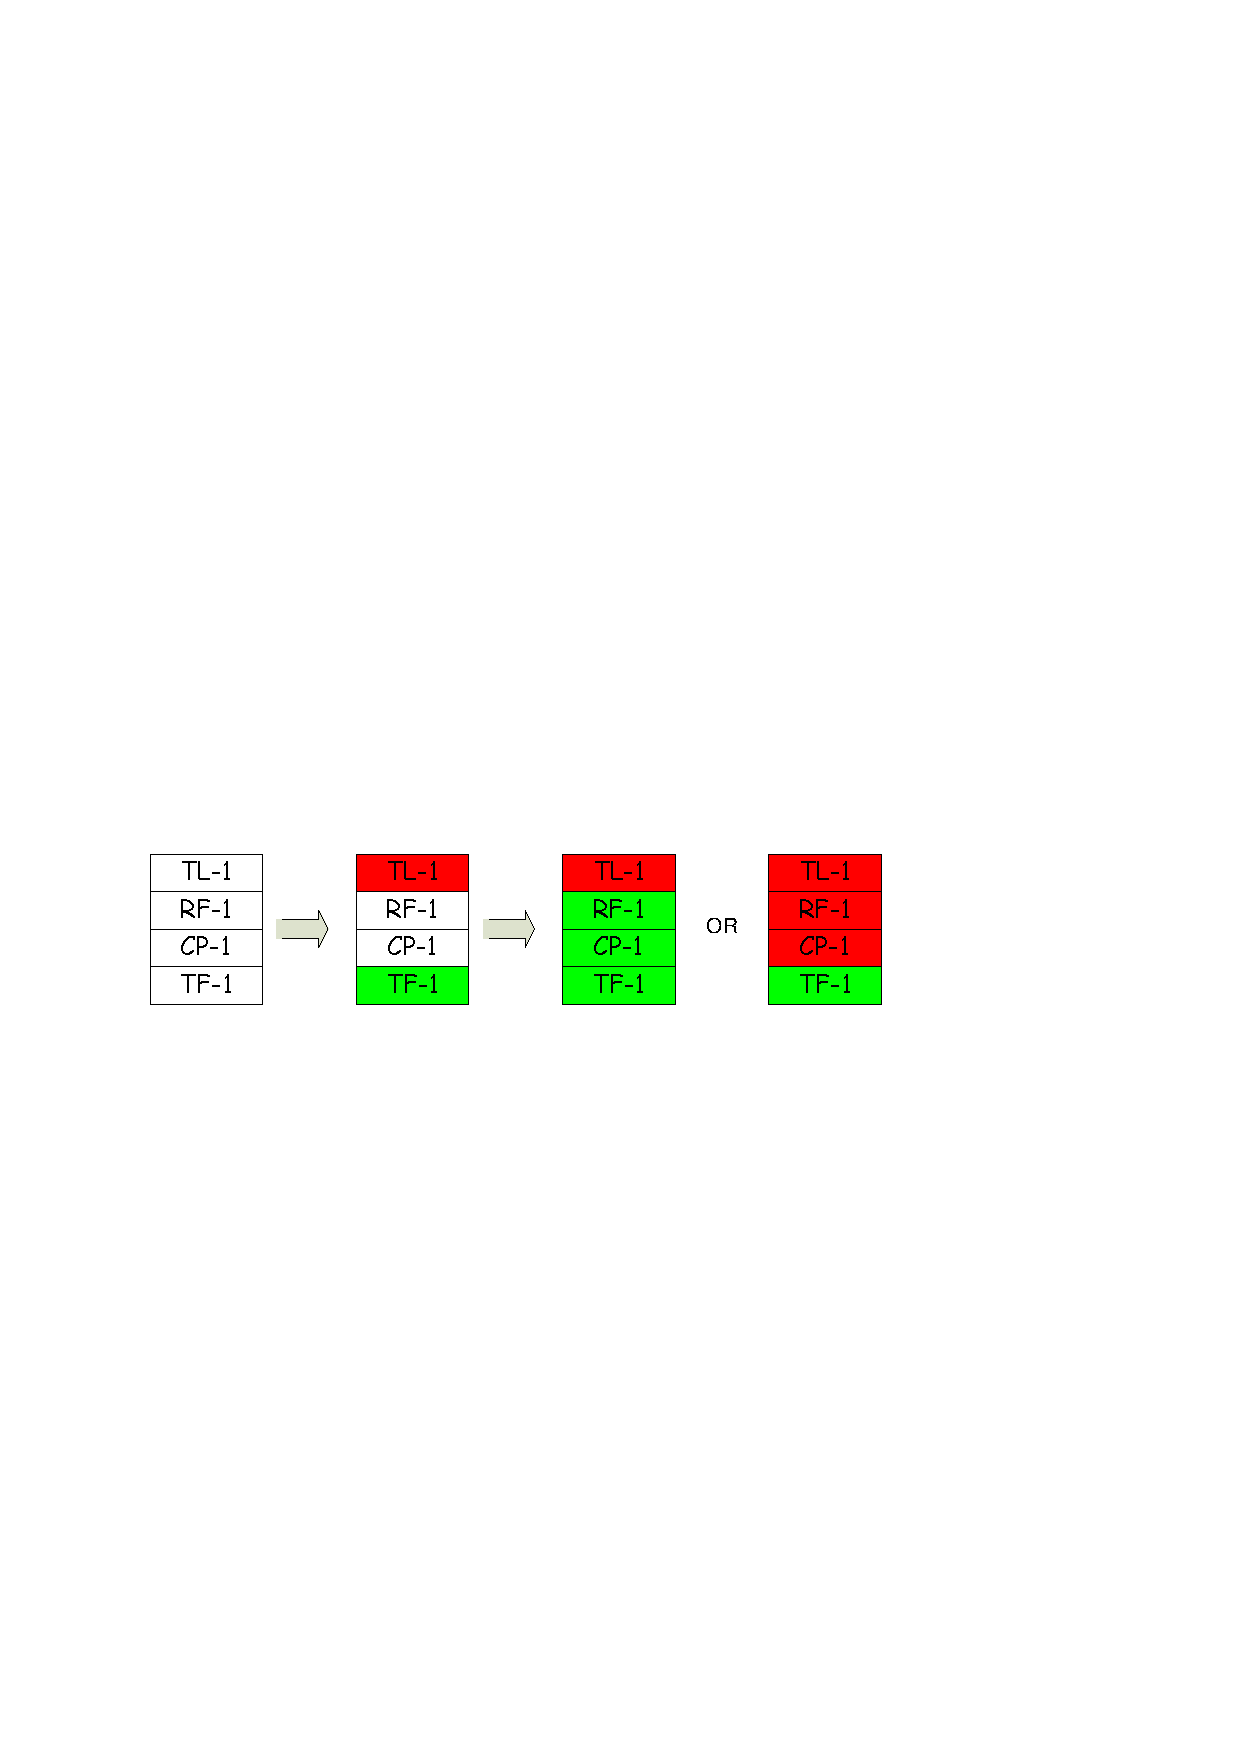
\includegraphics[width=0.6\textwidth]{figs/Visio-Zorro-Heuristic}
  \caption{Optimistic and Pessimistic Heuristic Algorithms}
  \label{fig:Zorro-HeuristicAlgorithm}
\end{figure}
Again, an episode is painted with green background if it is TDD 
conformant, otherwise it is painted with red background. Both of 
heuristics are supported by Zorro. In default, the optimistic
one is used, but Zorro allows developers to switch to the 
pessimistic heuristic.

\subsection{Zorro's TDD Episode Inference}
With episode categorization and TDD conformance heuristics, both 
of which are supported by the rule-based system, Zorro can automate
the recognition of TDD. 
%In addition, it can also differentiate TDD  from other development 
% methods, such as Test Last Programming. 
I conducted the ``TDD Episode Inference'' analysis using a real TDD 
development stream to demonstrate the Zorro's inference result. 
\begin{figure}[htbp]
  \centering
  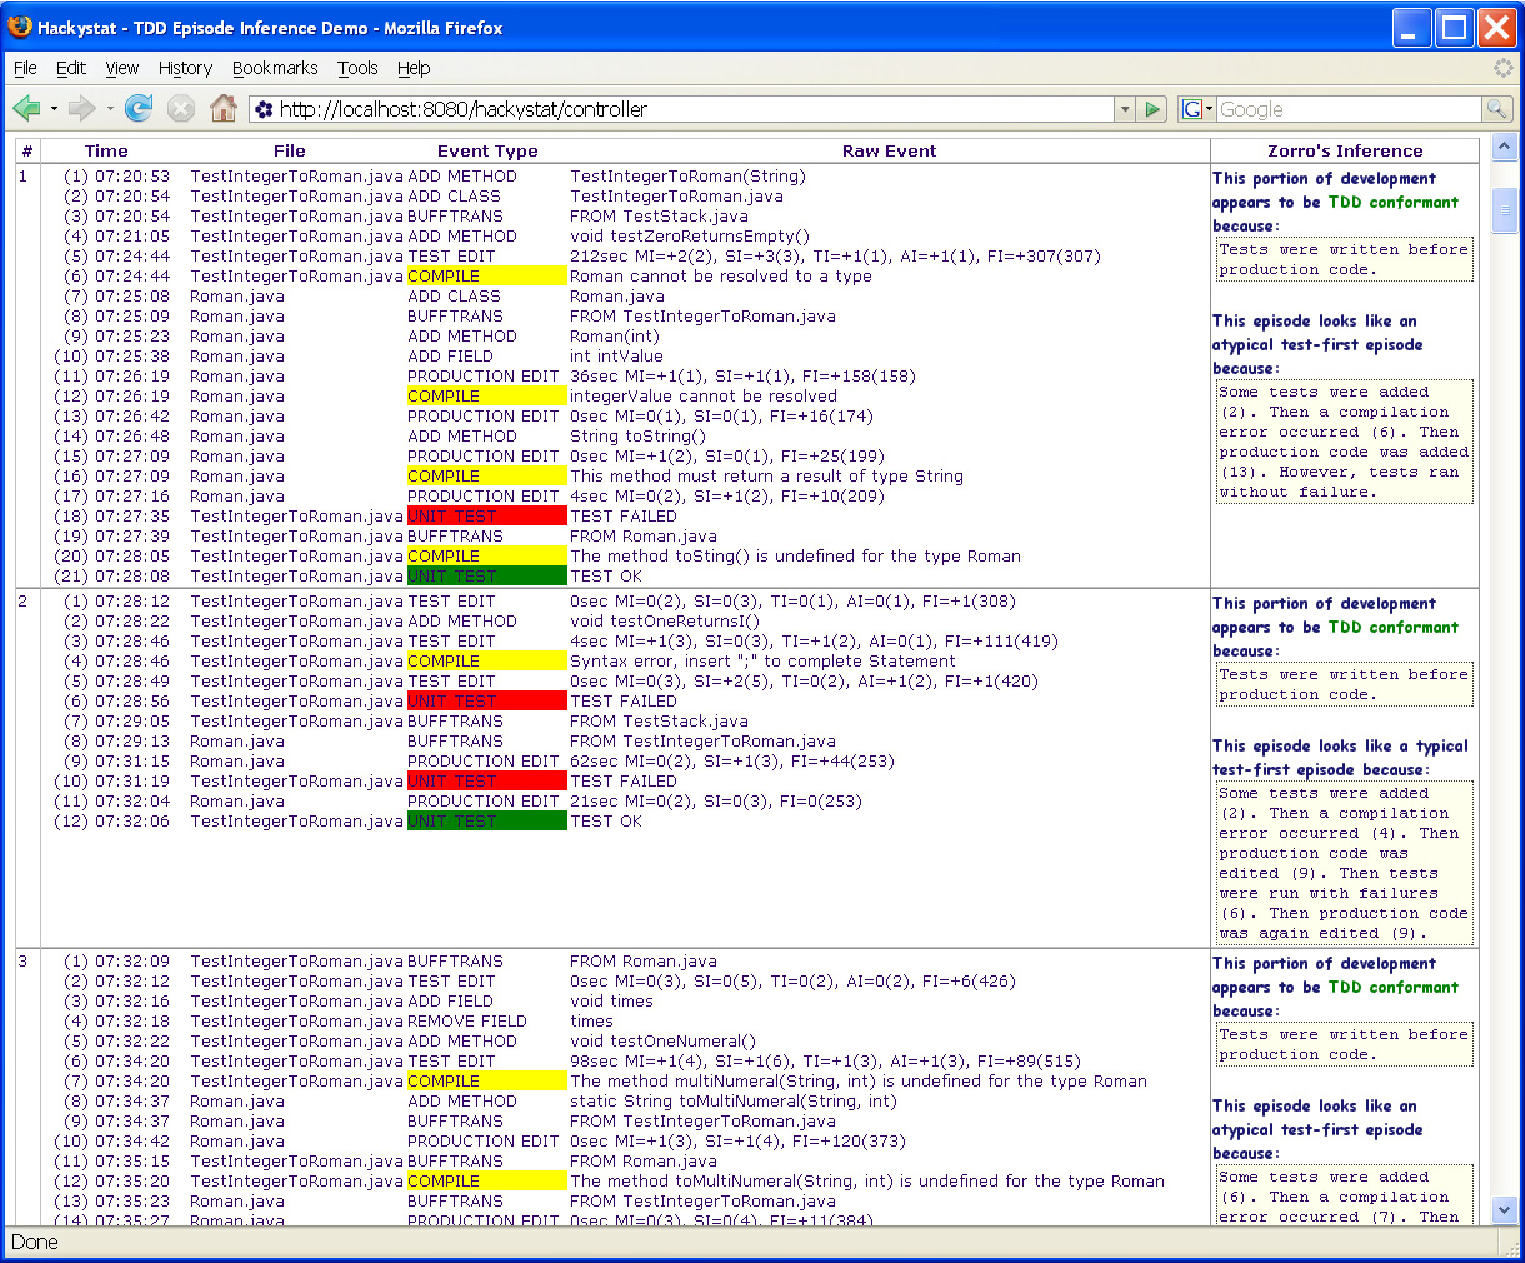
\includegraphics[width=0.9\textwidth]{figs/Zorro-Result-Demo}
  \caption{Demo of TDD Conformance Inference}
  \label{fig:Zorro-Process-Demo}
\end{figure}
An experienced developer solved the Roman numeral conversion problem 
(see Appendix \ref{app:UserStoriesRomanNumeral}) using TDD in the 
Eclipse IDE. The Hackystat Eclipse sensor was installed to instrument 
the development process for collecting development activities. Zorro 
partitioned his development stream into 16 episodes, and inferred 
his development behaviors. The screen-shot in 
Figure \ref{fig:Zorro-Process-Demo} shows the first three episodes 
with inferred development behaviors. They are all types of 
``Test First'' and conformant to TDD according to Zorro's inference.

This analysis is useful at demonstrating to new users how Zorro infers 
development behaviors. Another use of this analysis is 
to validate the correctness of Zorro's inference results. I will show 
how I enhanced this analysis for Zorro's validation in 
Chapter \ref{ch:Classroom}. Next, I will introduce Zorro's 
extensions to Hackystat's functionalities.

\section{Extensions to Hackystat's Functionalities}
TDD conformance is very important according to the discussion of related 
work in Chapter \ref{ch:RelatedWork}, and therefore I implemented 
the Zorro software system to provide explicit support for process 
conformance. Besides TDD conformance, 
with the capability of automated inference of TDD behaviors, more 
useful analyses that once were very hard can be conducted now. In 
the course of my research, I implemented TDD analyses including
``Episode Demography'', ``T/P Effort Ratio'', and 
``Episode Duration Distribution'' etc., for studying TDD 
(see Section \ref{sec:Zorro-Analysis}). Moreover, with the aid 
of Software project telemetry infrastructure, I implemented TDD 
telemetry reducers to assist research and management of software 
development in TDD (see Section \ref{sec:Zorro-Analysis-Telemetry}). 

\subsection{TDD Analyses}
\label{sec:Zorro-Analysis}
The following Zorro analyses have been developed to study software 
development in TDD and other development methods that include
unit testing.

% With our experiences, I have designed a set of analysis to understand
% an individual's practices of TDD. 
\subsubsection{Episode Demography}
The episode demography analysis provides an overview of a programming 
session as shown in Figure \ref{fig:Zorro-Analysis-EpisodeDemography}. 
\begin{figure}[htbp]
  \centering
  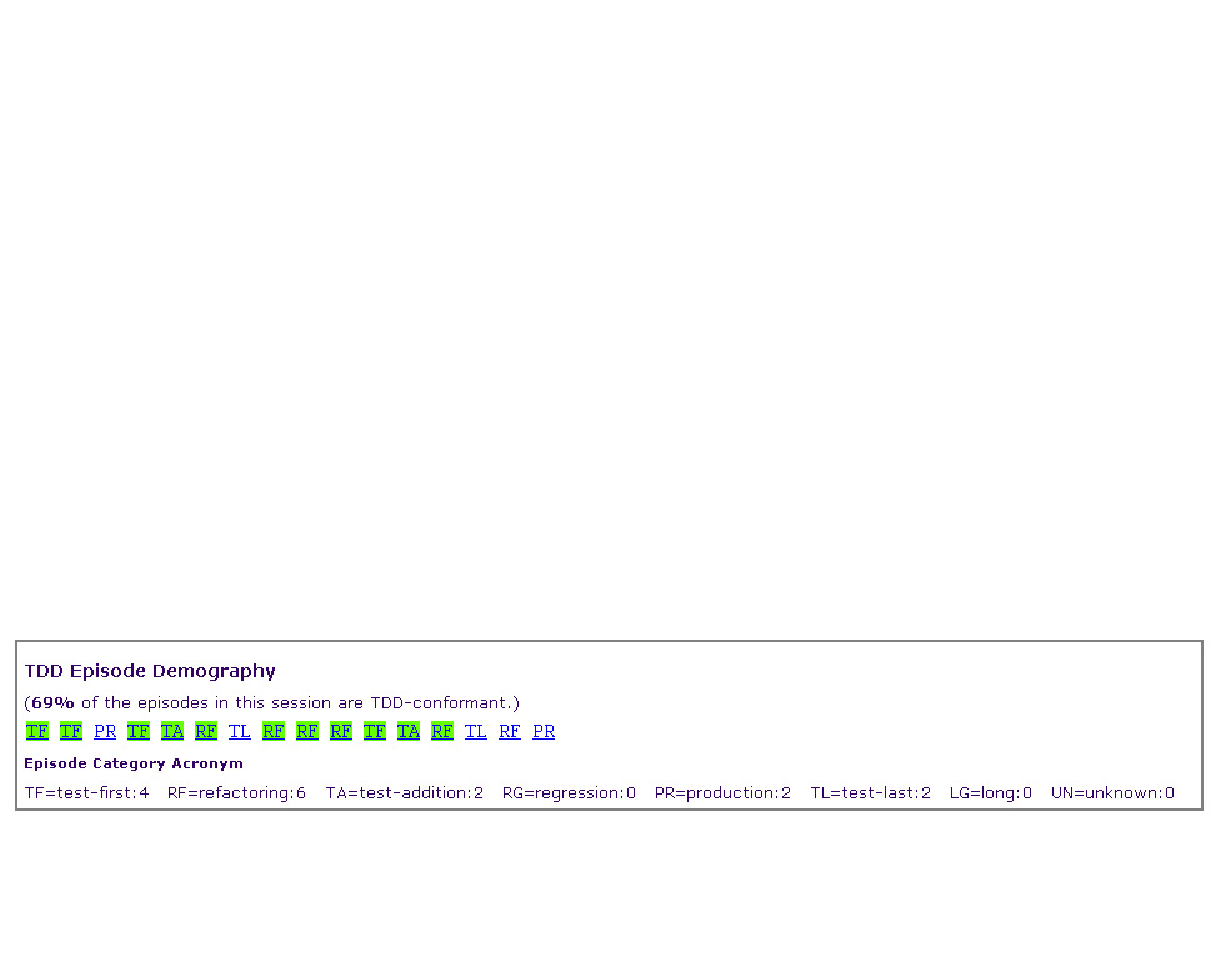
\includegraphics[width=1.0\textwidth]{figs/Zorro-Analysis-EpisodeDemography}
  \caption{Episode Demography Analysis}
  \label{fig:Zorro-Analysis-EpisodeDemography}
\end{figure}
In Figure \ref{fig:Zorro-Analysis-EpisodeDemography}, each small 
box with a two-letter acronym represents an episode. The legend
explains the links between two-letter episode acronyms and episode types. 
The background color of an episode tells its TDD conformance. 
If the episode is TDD conformant, the background is green; otherwise 
it is transparent. Episodes are clickable in the actual analysis. 
Clicking on an episode takes users to another analysis that is 
similar to the one illustrated in Figure \ref{fig:Zorro-Process-Demo}. 

Some useful information can be obtained using the episode demography
analysis. For instance, the example presented in Figure 
\ref{fig:Zorro-Analysis-EpisodeDemography} shows that this programming
session has 17 episodes, of which 69\% are TDD conformant. Four
episodes are ``Test First'', six are ``Refactoring'', and 
two are ``Test Last''. This information can be used to 
improve TDD conformance. If a higher degree of TDD conformance
is wanted, developers can study what are the legitimate TDD episodes 
to improve their compliance with TDD. Moreover, this analysis
can also be used to find development patterns. For instance, in
Figure \ref{fig:Zorro-Analysis-EpisodeDemography}, we can observe 
two patterns (TF)(TA)+ and (TA)(RF)+. The pattern (TF)(TA)+ means that 
a ``Test First'' episode is followed by one or more ``Test Addition''
episodes. The (TA)(RF)+ means that a ``Test Addition'' episode is 
followed by one or more ``Refactoring'' episodes.

\subsubsection{T/P Effort Ratio}
Unlike ``Episode Demography'', the ``T/P Effort Ratio'' analysis is not 
directly derived from Zorro's inference. In Section \ref{sec:Zorro-Hackystat},
we discussed that Zorro extends Hackystat's data collection. One 
extension is that it requires numbers of test methods and assertion 
statements. With this information, we can easily tell if a developer 
is working on test code at a given time. The T/P Effort
Ratio stands for the effort a developer spent on test code, 
compared to the effort spent on production code. 
Figure \ref{fig:Zorro-Analysis-TPEffortRatio} shows an example
of the T/P Effort Ratio analysis using the same TDD programming 
session used in Figure \ref{fig:Zorro-Analysis-EpisodeDemography}.
\begin{figure}[htbp]
  \centering
  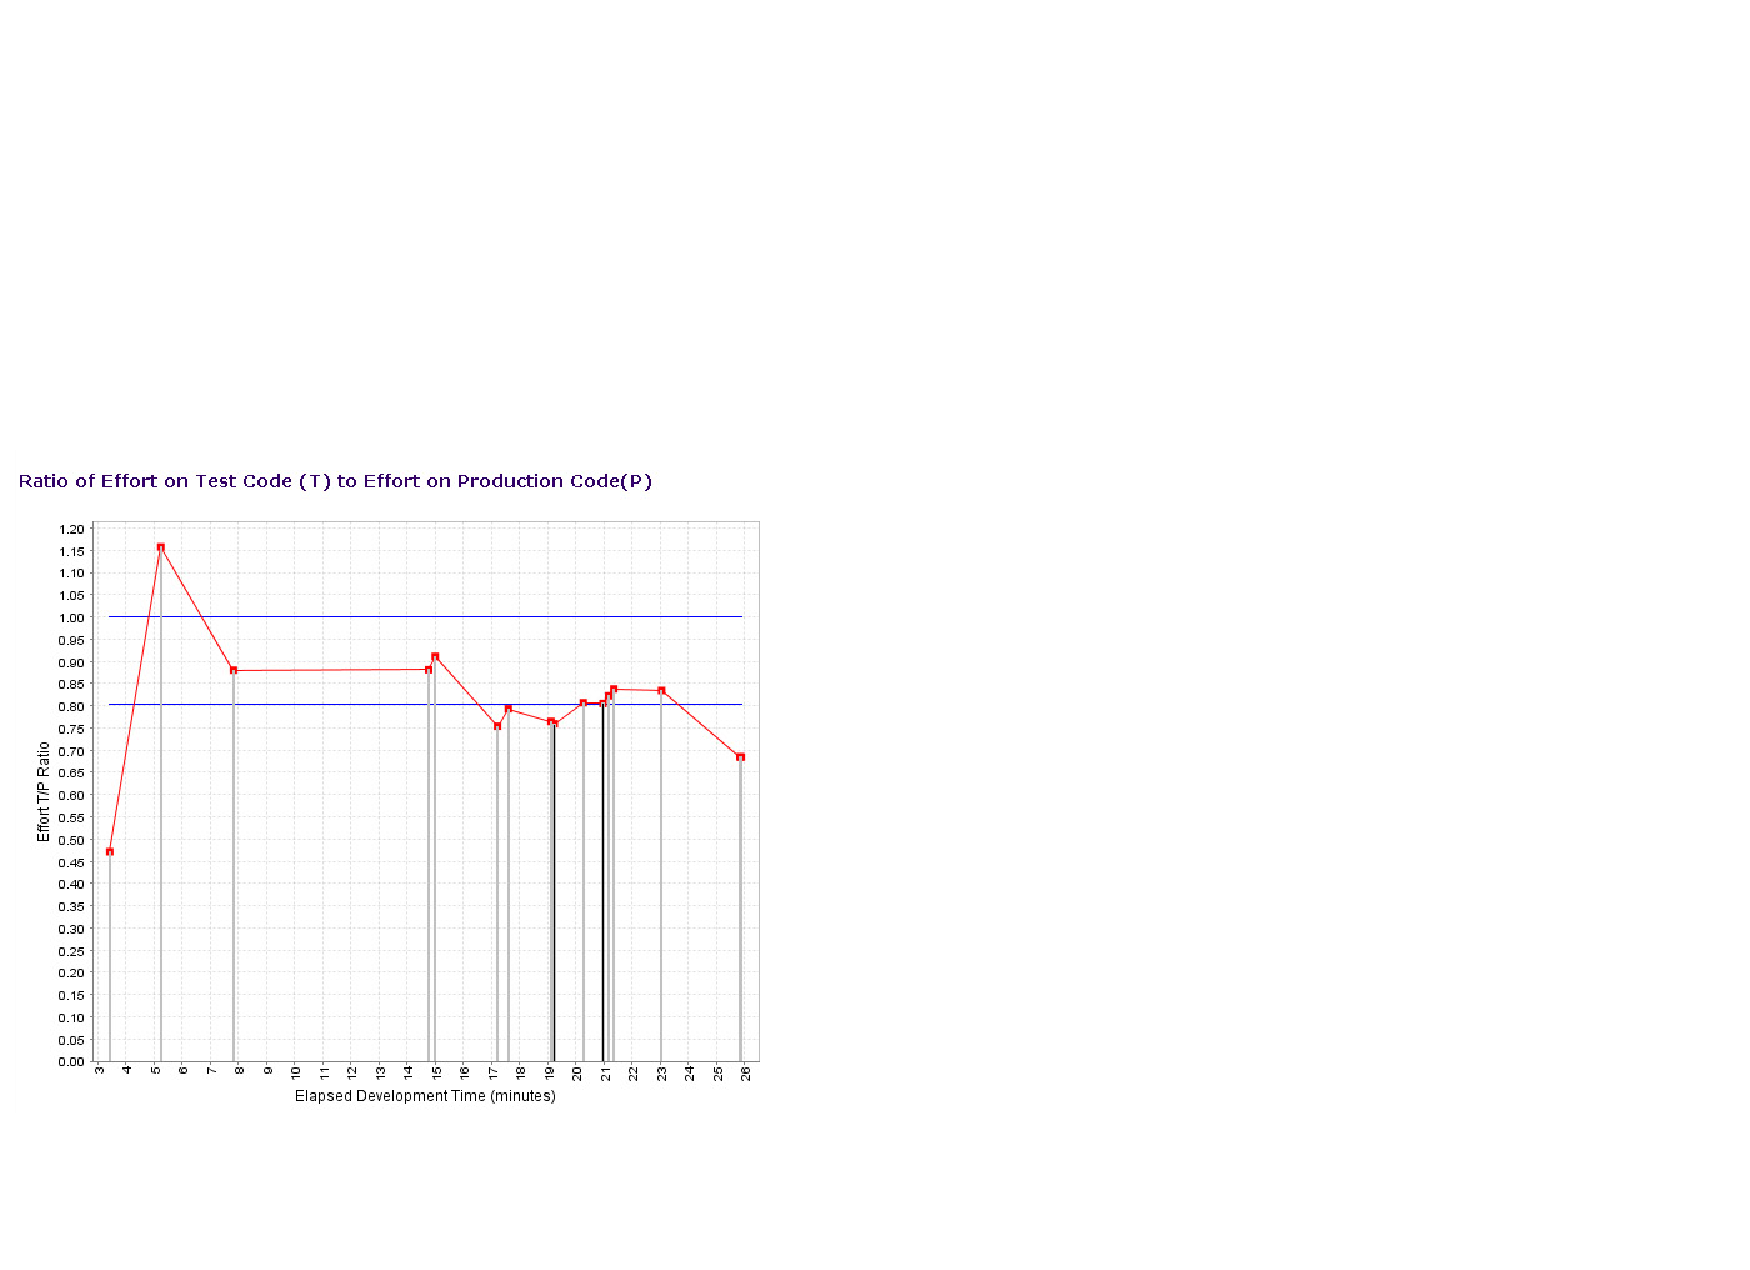
\includegraphics[width=0.7\textwidth]{figs/Zorro-Analysis-TPEffortRatio}
  \caption{Test Effort vs. Production Effort}
  \label{fig:Zorro-Analysis-TPEffortRatio}
\end{figure}
In Figure \ref{fig:Zorro-Analysis-TPEffortRatio}, the horizontal axis
is the elapsed development time in minutes, and the vertical axis is
the ratio of effort spent on test code to effort spent on production
code. The T/P ratio over 1.0 indicates more effort on writing
test code than on writing production code. The vertical bars are
episode borders, thus, the span between bars can represent episode 
durations.  

The example illustrated in Figure 
\ref{fig:Zorro-Analysis-TPEffortRatio} shows that the effort spent on
testing code is consistent over the course of this TDD development session. 
Approximately, on average, effort on testing code is about 80\% of effort
on production code. This analysis can be applied to not only TDD but also 
other development methods that include unit testing. An interesting use 
of it would be to compare T/P effort ratio differences between TDD and 
Test Last Programming. 

\subsubsection{T/P Size Ratio}
Same as the T/P Effort Ratio analysis, the T/P Size Ratio analysis is also
based upon Zorro's extension to Hackystat's data collection. In Table 
\ref{tab:Zorro.Sensors}, we have shown that the Zorro compatible sensor 
collects size information (current-size, mostly line of code) for both
of test and production code. With this information, we can compute the
incremental changes of test code size, production code size, and the 
ratio of the two. Figure \ref{fig:Zorro-Analysis-TPSizeRatio} shows 
an example of the T/P Size Ratio analysis using the same TDD programing 
session. 
\begin{figure}[htbp]
  \centering
  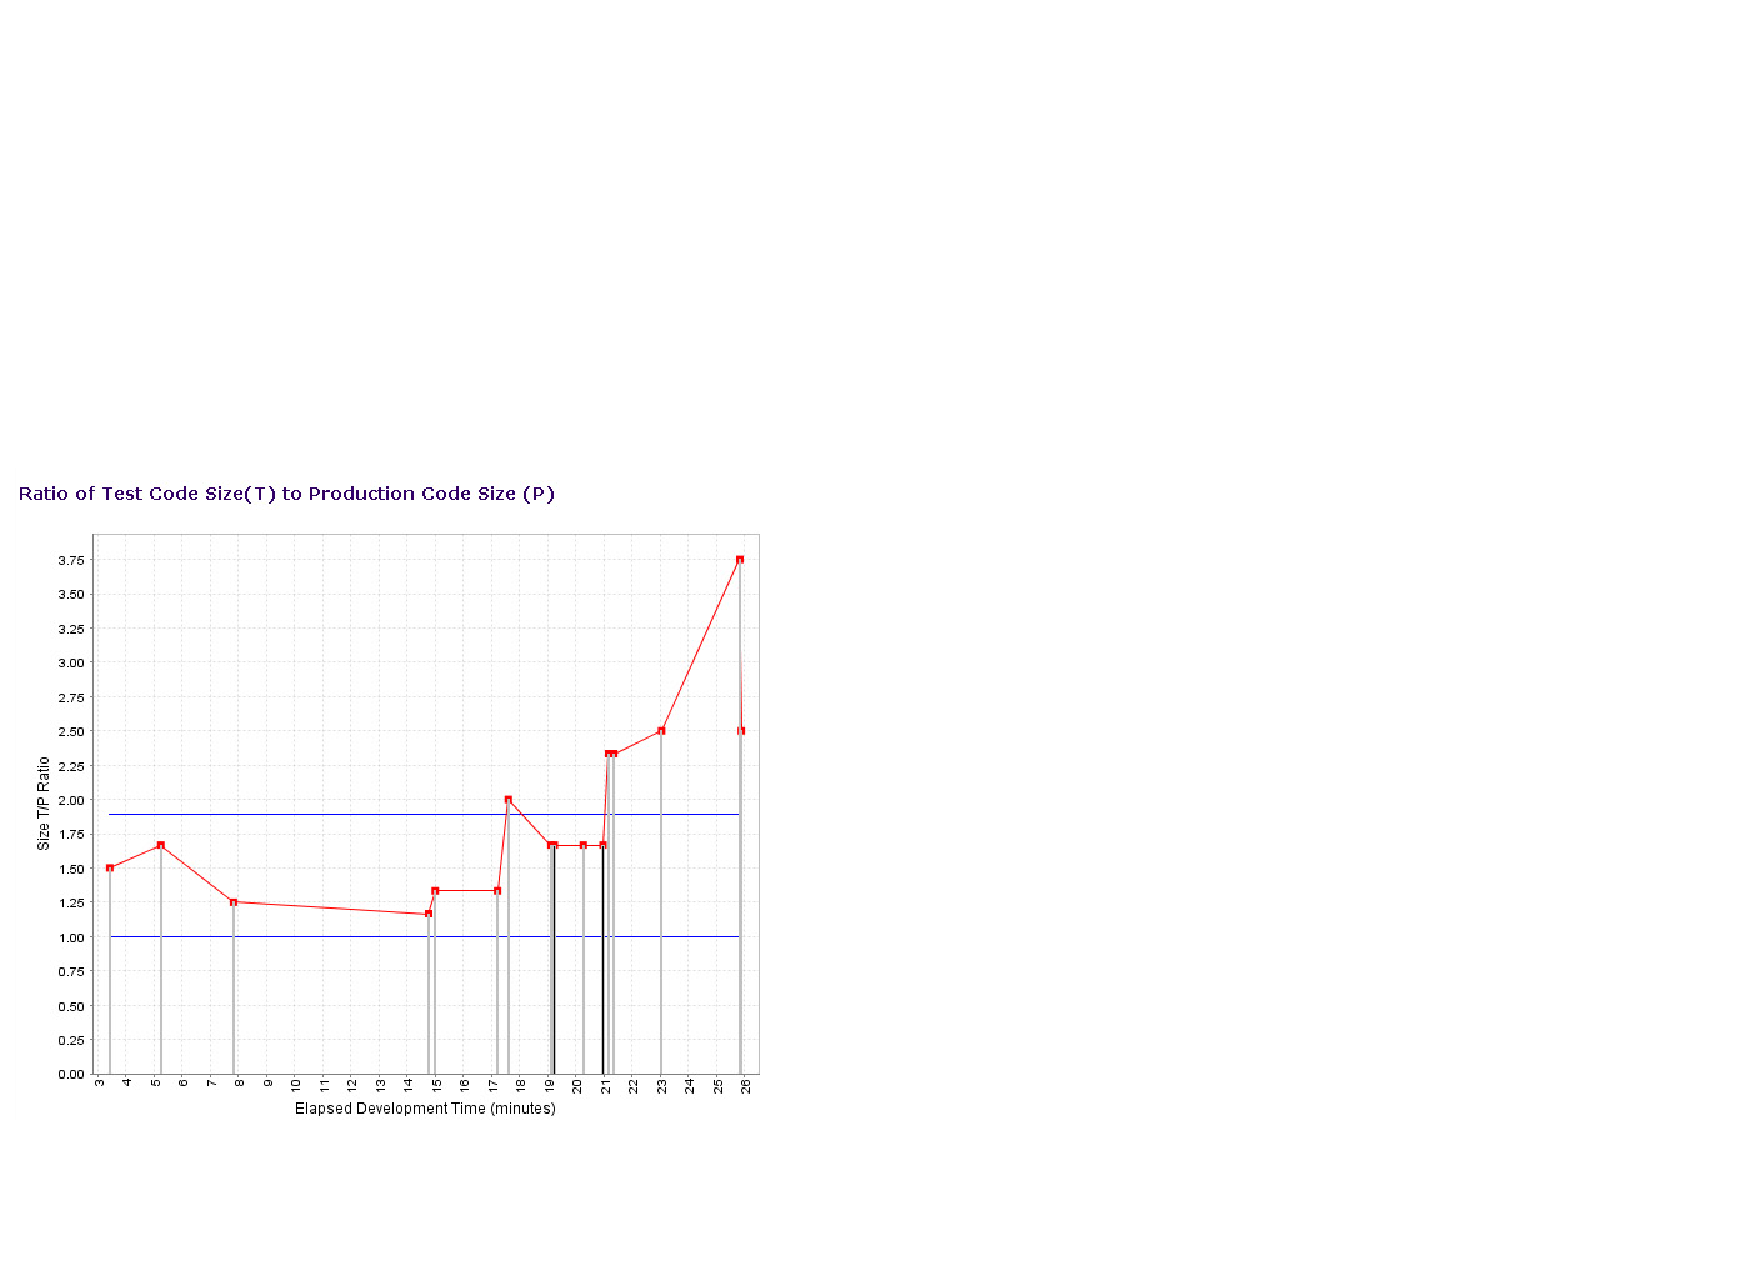
\includegraphics[width=0.7\textwidth]{figs/Zorro-Analysis-TPSizeRatio}
  \caption{Test Size vs. Production Size}
  \label{fig:Zorro-Analysis-TPSizeRatio}
\end{figure}
The interpretation to this analysis is exactly the same to Figure
\ref{fig:Zorro-Analysis-TPEffortRatio}, except that each value 
in Figure \ref{fig:Zorro-Analysis-TPSizeRatio} is the ratio of 
test code size to production code size. 

The example illustrated in Figure \ref{fig:Zorro-Analysis-TPSizeRatio}
shows that test code is always more than production code. Again, this
analysis is applicable to any development methods where unit testing 
is practiced. 

\subsubsection{Episode Duration}
The Episode Duration analysis is inspired by TDD's characteristically 
short durations that I discussed in Section \ref{sec:related-tdd}. How
frequently unit tests are invoked is an alternative indicator of 
TDD conformance \cite{Wang:04}. Figure \ref{fig:Zorro-Analysis-EpisodeDuration}
shows an example of the Episode Duration analysis. 
\begin{figure}[htbp]
  \centering
  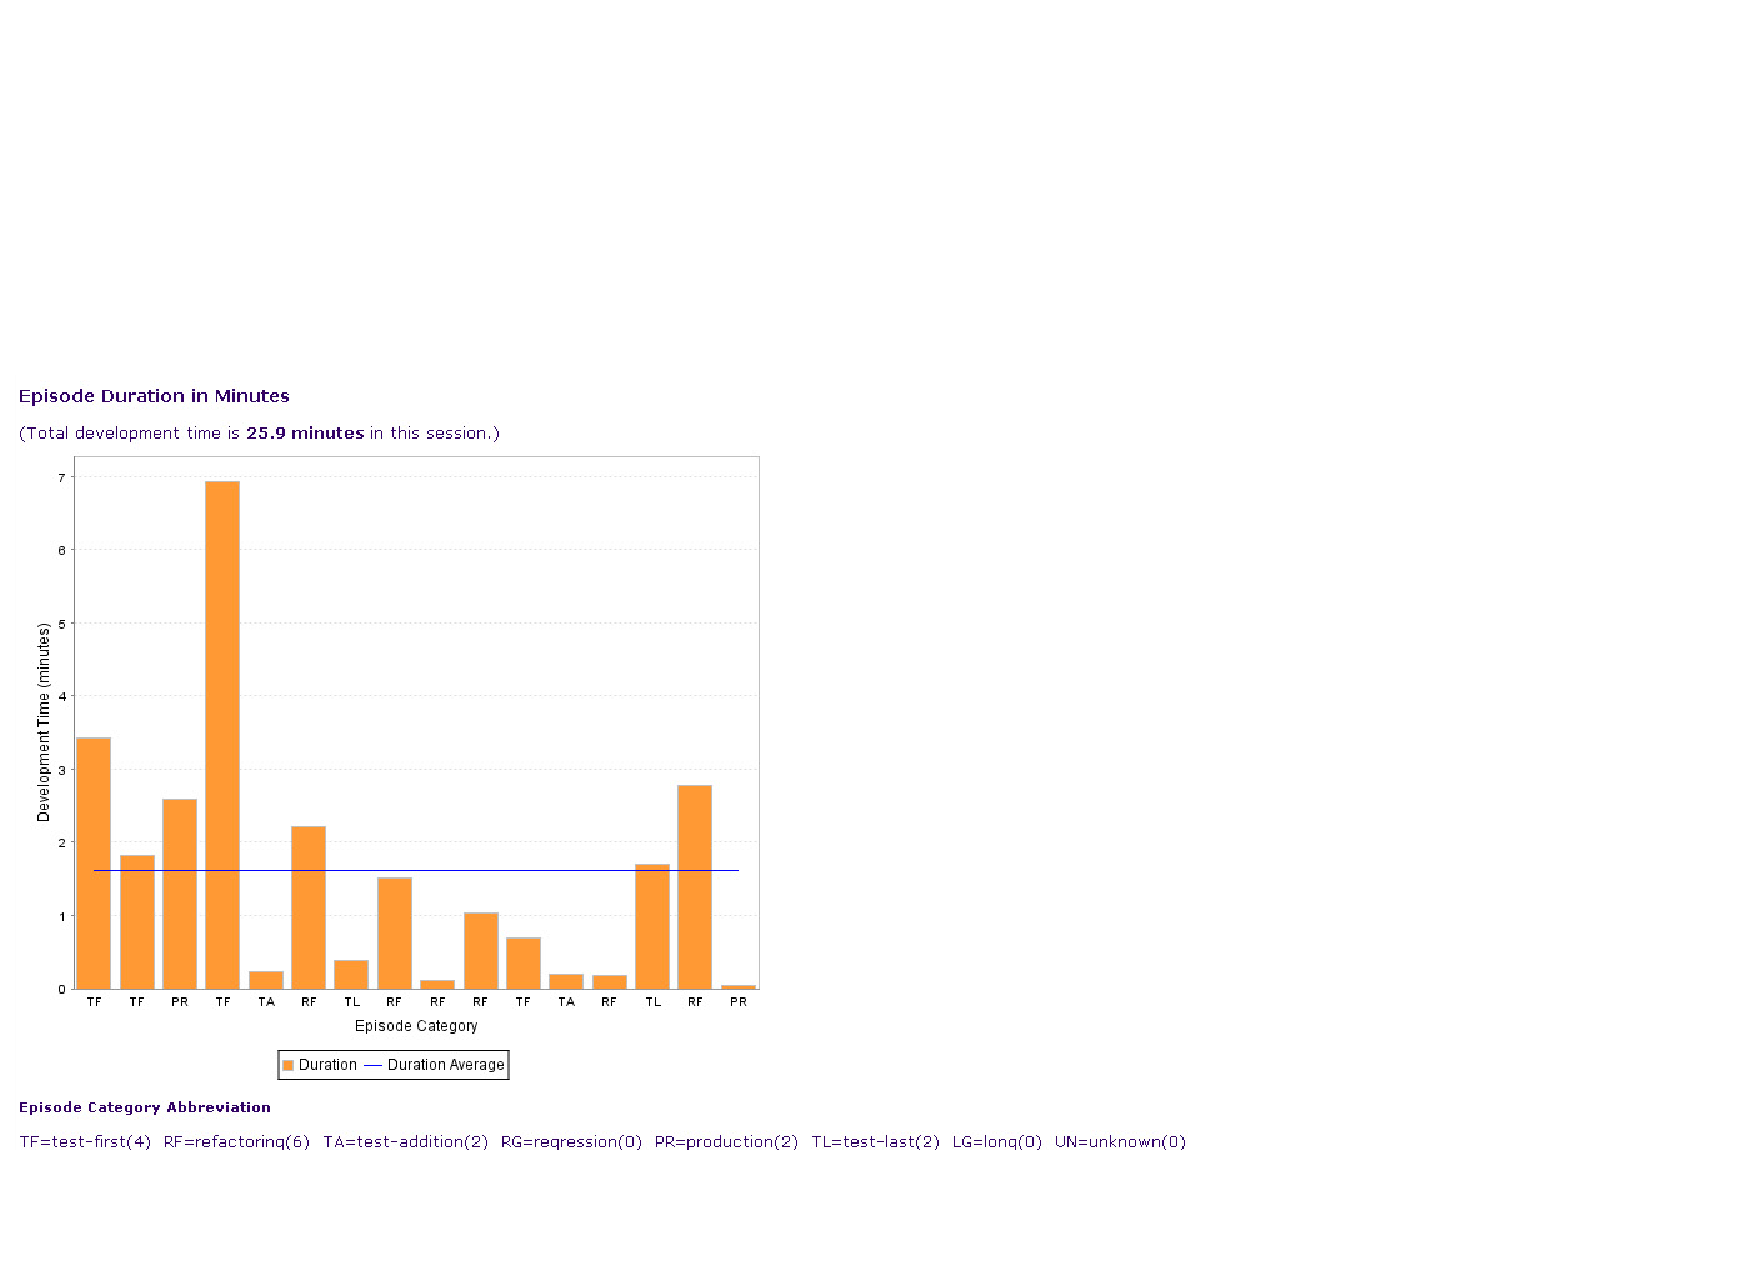
\includegraphics[width=0.7\textwidth]{figs/Zorro-Analysis-EpisodeDuration}
  \caption{Episode Duration}
  \label{fig:Zorro-Analysis-EpisodeDuration}
\end{figure}
The interpretation of this analysis is very straightforward. The 
horizontal axis has the two-letter acronym for each episode. 
The vertical axis is the episode duration in minutes. As we 
can see in Figure \ref{fig:Zorro-Analysis-EpisodeDuration},
with a little hill climbing at the beginning, tests were invoked 
frequently in this TDD programming session. 

Similarly, this analysis is applicable to any development methods 
where unit testing is practiced.  The durations in Figure 
\ref{fig:Zorro-Analysis-EpisodeDuration} are mostly short, which
supports the short duration claim made about TDD iterations. In 
practice, I rarely observed episodes that were longer than 30 minutes
in duration. In that case, the conformance to TDD is likely not 
stringent any more. A tabular report 
(Table \ref{tab:Zorro-Analysis-EpisodeDurationTable}) is also 
available for comparing episode duration differences among 
episode categories. 
\begin{table}[htbp]
\centering
  \caption{Duration Average by Episode Category}
  \begin{tabular}{|l|l|} \hline 
  Category  &   Average Duration (minutes) \\ \hline
  TF    & 3.2 \\ \hline
  RF    & 1.3 \\ \hline
  TA    & 0.2 \\ \hline
  RG    & 0   \\ \hline
  PR    & 1.3 \\ \hline
  TL    & 1  \\ \hline
  LG    & 0  \\ \hline
  UN    & 0 \\ \hline
  \end{tabular}
  \label{tab:Zorro-Analysis-EpisodeDurationTable}
\end{table}
 
\subsubsection{Episode Duration Bin}
The Episode Duration analysis lines up episodes with their 
durations, which is useful at displaying progressive changes. 
An alternative presentation is to arrange episodes with
close durations into a bin. Figure 
\ref{fig:Zorro-Analysis-EpisodeDurationBin} is an example
showing the Episode Duration Bin analysis. 
\begin{figure}[htbp]
  \centering
  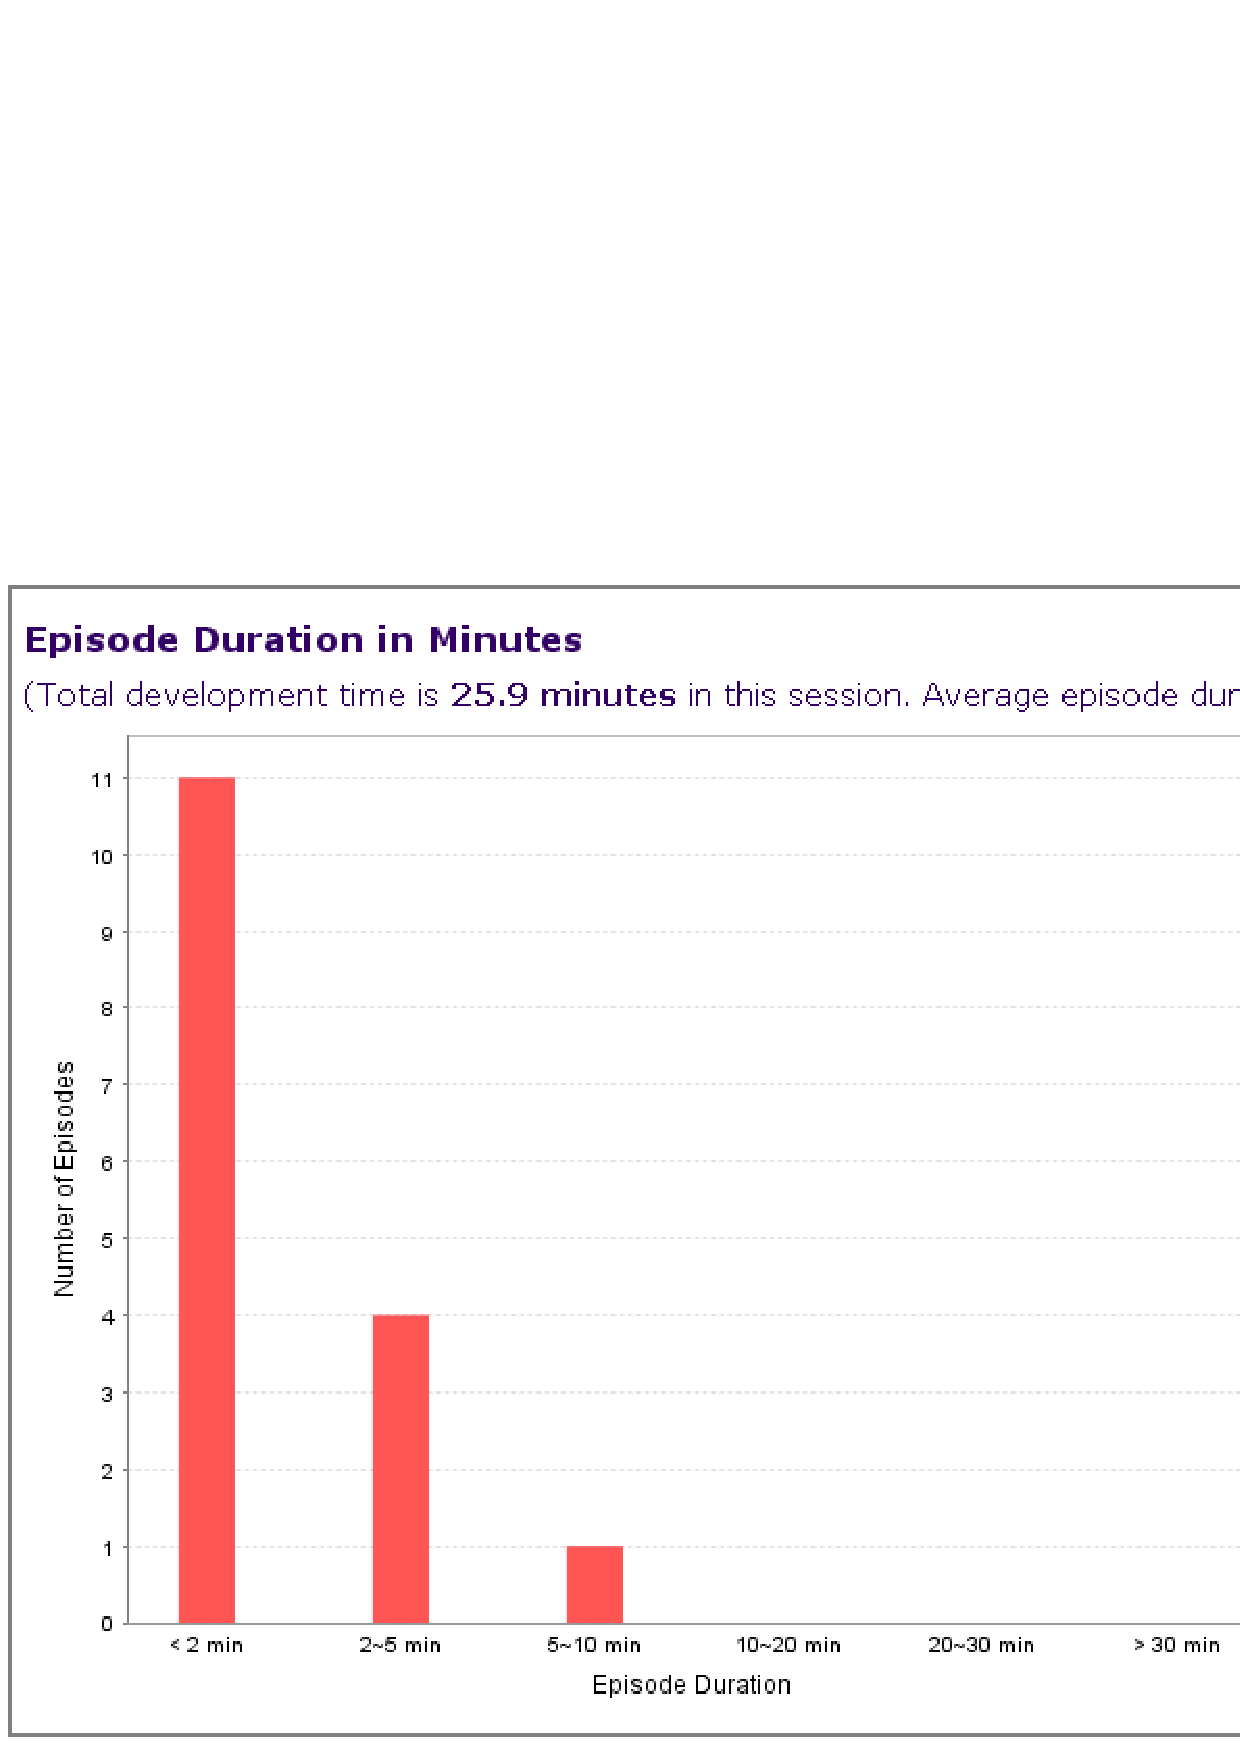
\includegraphics[width=0.7\textwidth]{figs/Zorro-Analysis-EpisodeDurationBin}
  \caption{Episode Duration Bin}
  \label{fig:Zorro-Analysis-EpisodeDurationBin}
\end{figure}
In Figure \ref{fig:Zorro-Analysis-EpisodeDurationBin}, the horizontal 
axis has a set of bins of episode durations, and the vertical axis 
is the number of episodes. 

Similar to the Episode Duration analysis, this analysis can be used to
verify TDD's short duration characteristic. An ideal TDD development 
session should have many short episodes with no or very few long episodes. 
If too many long episodes are observed, perhaps developers should take 
actions to develop and run tests more frequently. An episode duration 
distribution table (see Table \ref{tab:Zorro-Analysis-EpisodeDistribution})
is attached to this analysis.
\begin{table}[htbp]
\centering
  \caption{Episode Duration Distribution by Category}
  \begin{tabular}{llllllll} 
        Category & \textless 2 min & 2\~{}5 min & 5\~{}10 min & 10\~{}20 min & 20 \~{}30 min & \textgreater 30 min & Total \\ \hline
  TF      &  2  &  1 &   1  &  &        &  &  4  \\ 
  RF      &  4  &  2 &                  &  &    &  &    6  \\ 
  TA      &  2  &        &                      &  &    &  &    2  \\ 
  RG      &             &        &      &  &  &  &  0  \\ 
  PR      &  1  &  1 &                  &  &  &  &      2  \\ 
  TL      &  2  &        &                      &  &  &  &      2  \\ 
  LG      &     &        &                      &  &  &  &      0  \\ 
  UN      &             &        &                      &  &  &  &  0  \\ \hline
  Total &  11 &  4 &    1       & 0 & 0 & 0 &   16  \\  
  \end{tabular}
  \label{tab:Zorro-Analysis-EpisodeDistribution}
\end{table}

\newpage
\subsection{TDD Telemetry Streams}
\label{sec:Zorro-Analysis-Telemetry}
The analyses in Section \ref{sec:Zorro-Analysis} leverage
Zorro's recognition of TDD development behaviors. They can be used
to understand and improve TDD development for individuals. In order
to support project management and improvement, I implemented a
group of TDD telemetry streams in my research. Because Zorro 
abstracts software metrics into low-level development behaviors, 
the synergy of Zorro and Software telemetry allows better management 
of software projects developed in TDD. In this section, I will 
introduce Software telemetry, and present TDD telemetry analyses. 

\subsubsection{Software Project Telemetry and TDD Telemtry Reducers}
The Software project telemetry \cite{csdl2-04-11,csdl2-06-05} was 
developed by Qin Zhang in the Collaborative Software Development 
Lab at the University of Hawaii. It is an infrastructure to aggregate 
metrics data together to perform daily, weekly, or monthly analyses 
to support in-process software project management and decision makings. 
Software telemetry abstracts software metrics into streams, charts and 
reports. The telemetry stream contains a series of time-stamped events 
in the daily, weekly, or monthly granularity. The telemetry charts and 
reports provide visualization of telemetry streams. Detecting changes 
and covariance in the trend of telemetry streams enables an incremental, 
visible, and experimental approach to manage software 
projects \cite{csdl2-06-05}. 

The telemetry reducer is the extension point of Software telemetry, 
which can be used to extend the existing telemetry stream base.  
The following lists TDD telemetry reducers supplied in Zorro.
\begin{itemize}
\item \textbf{TDDPercent Reducer}:\\
Computes a single telemetry stream for percentage of TDD development 
time to overall development time. Alternatively, the percentage 
can also be the number of TDD compliant episodes to the number of 
total episodes. 

\item \textbf{TDDProductionDevTime Reducer}:  \\
Computes a single telemetry stream of development time on 
production code. Though its name suggests that this reducer 
is for TDD, it can actually be applied to other development 
methods as well.

\item \textbf{TDDTestDevTime Reducer}: \\
Computes a single telemetry stream of development time on
test code. Same as TDDProductionDevTime, it can be applied 
to development methods other than TDD if unit testing is 
used. 

\item \textbf{TDDDevTime Reducer}: \\
Computes a single telemetry stream of total development time. 
Note that Software telemetry already defines a DevTime, which
is different from TDDDevTime. The TDDDevTime can be 
thought as the summation of development time on production,
test, and others such as XML configuration files. 

\item \textbf{EpisodeAverageDuration Reducer}: \\
Computes a single telemetry stream of average episode duration.
It can be applied to TDD and other development methods. It 
indicates how frequently unit test is invoked. 

\item \textbf{TDDMemberProductionDevTime Reducer}: \\
Computes multiple telemetry streams for development time on
production code, one telemetry stream for each project member.

\item \textbf{TDDMemberTestDevTime Reducer}: \\
Computes multiple telemetry streams for development time on
test code, one telemetry stream for each project member.

\item \textbf{TDDMemberDevTime Reducer}: \\
Computes multiple telemetry streams for total development time, 
one telemetry stream for each project member.

\item \textbf{MemberEpisodeAverageDuration Reducer}: \\
Computes multiple telemetry streams for average episode durations, 
one telemetry stream for each project member.

\end{itemize}

\subsubsection{TDD Telemetry Analyses}
The availability of TDD telemetry reducers enables developers to 
invoke telemetry analyses using Zorro's recognized 
low-level development behaviors. 

Recall that a benefit of TDD is that the code developed in TDD
should be 100\% covered because no functional code is created
without a unit test (see Section \ref{sec:related-tdd}). So it 
would be interesting to study this claim. Since Zorro has the
TDDPercent Reducer, we can define a telemetry stream
reporting percentages of TDD development and correlate it with
the test coverage stream that is already included in Software
telemetry(Page 59 \cite{csdl2-06-05}). The following code
is a definition of the telemetry stream and chart for this
investigation.
\begin{verbatim}
  streams TDDPercent(type) = {
    "Percentage of Test-Driven Development", 
    TDDPercent(type) * 100
  };

  chart TDD-Coverage-Percentage-Chart() = {
    "Percentage of TDD Episodes (time) and Coverage", 
    (TDDPercent("time"), percentageYAxis("TDD \%")),
    (Coverage-Percentage("**", "line"), 
     percentageYAxis("Coverage \%"))
  };
\end{verbatim}

Figure \ref{fig:Zorro-Analysis-TDDPercentCoverage} 
is a weekly telemetry chart showing percentage of TDD development 
and test coverage.
\begin{figure}[htbp]
  \centering
  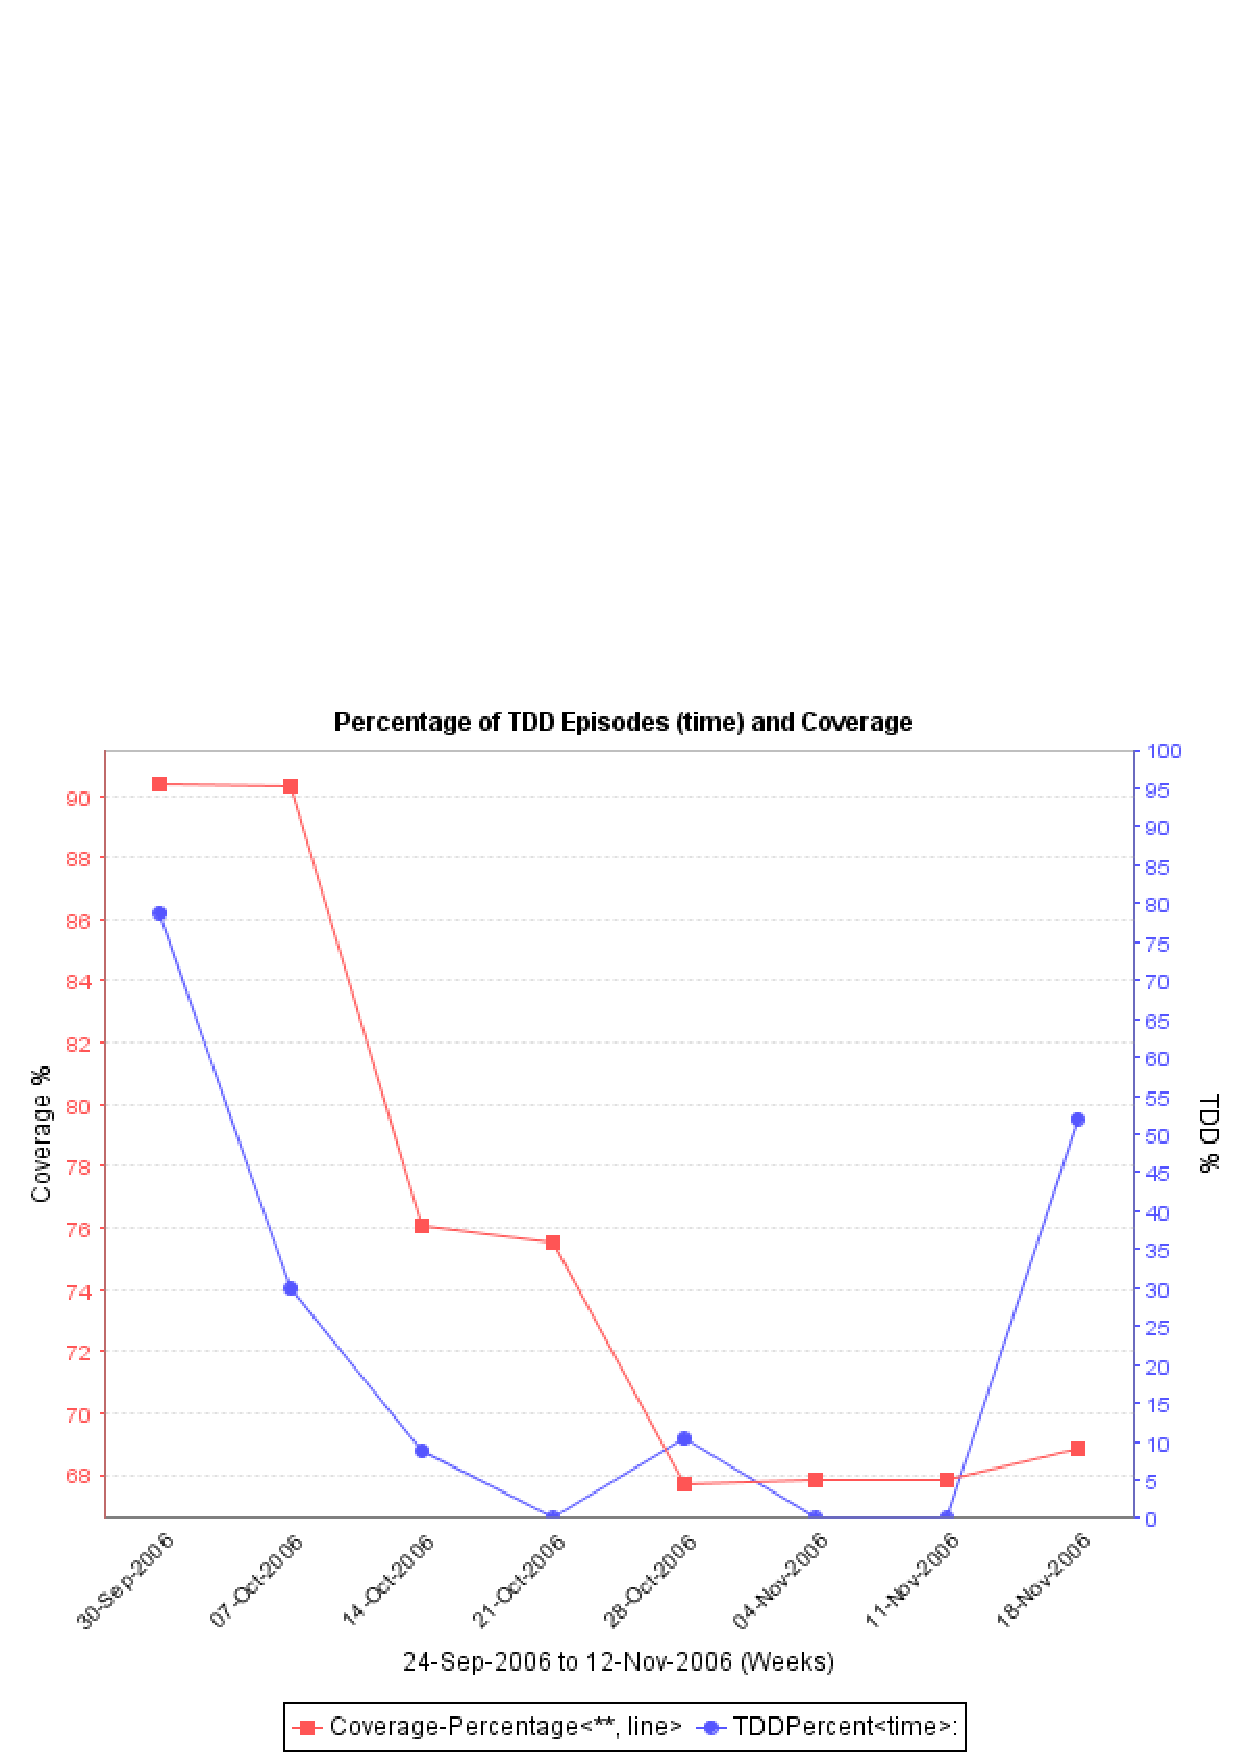
\includegraphics[width=0.8\textwidth]{figs/Zorro-TDD-Coverage}
  \caption{TDD Percentage and Testing Coverage}
  \label{fig:Zorro-Analysis-TDDPercentCoverage}
\end{figure}
From the week of Sep 30, 2006 to the week of Nov 18, 2006, I worked on the
Zorro software system and implemented Zorro's web validation interface.
Due to the fact that testing web interfaces requires a lot of additional
effort, my conformance to TDD dropped down significantly in that period. As
a result, the test coverage dropped from 90\% to below 70\% over the course
of eight weeks software development. Though we can not directly verify the
claim of 100\% test coverage characteristic of TDD, indeed the analysis
shows that deviating from TDD caused decrease of test coverage. In turn,
this indicates that TDD can help to improve test coverage.

\begin{comment}
The TDD telemetry reducers enable us to define telemetry streams
to monitor software project development.
\begin{figure}[htbp]
  \centering
  \includegraphics[width=0.8\textwidth]{figs/Zorro-Analysis-TDDPercent}
  \caption{Telemetry of TDD Percent}
  \label{fig:Zorro-Analysis-Telemetry-TDDPercent}
\end{figure}
\paragraph{Ratio of Effort on Test to Effort on Production}
\label{sec:RatioOfEffortOnTestToEffortOnProduction}

%% Tablelized chart. 
\paragraph{TDD Percentage vs. Testing Coverage}
\label{sec:TDDPercentageVsTestingCoverage}
\end{comment}

\section{Chapter Summary}
In this chapter, I introduced Zorro's implementation with the support 
of the Hackystat and SDSA frameworks. Zorro extends Hackystat's 
data collection, specializes SDSA's low-level development
behaviors inference for TDD, and supplies new functionalities to 
Hackystat. Zorro's development behaviors and conformance of TDD 
were detailed in this chapter, along with an introduction
to TDD analyses and telemetry reducers implemented in Zorro.